\documentclass[a4paper,10pt,oneside,openany]{book}

\usepackage[english]{babel}

\usepackage[utf8]{inputenc} % Consente l'uso dei caratteri accentati italiani
\usepackage[T1]{fontenc} % Consente l'uso di caratteri speciali appartenenti in genere ad alfabeti non inglesi

\usepackage{fancyhdr} % Consente il rendering della copertina

\usepackage{graphicx} % Consente l'inserimento delle figure nel documento

\usepackage{subfigure} % Consente l'inserimento di sottofigure

\usepackage{tabularx} % Consente l'uso di funzionalità aggiuntive alle tabelle
\usepackage{longtable} % Consente la scrittura delle tabelle su più pagine

\usepackage[titletoc]{appendix} % Consente di porre le appendici in indice

\usepackage{float} % Necessario per inserire immagini flottanti

\usepackage{fancyvrb} % Consente l'utilizzo di finestre Verbatim (testo cche si vuole porre così com'è, senza formattazione alcuna) all'interno di una cornice

\usepackage{amsmath} % Consente l'uso di funzioni aggiuntive per le formule
\numberwithin{equation}{section}

\usepackage{hyperref} % Indice degli argomenti e rimandi cliccabili, per una navigazione più comoda all'interno del file

\usepackage{lipsum} % Consente di inserire testo fittizio all'interno della tesi. Inutile in fase di scrittura della tesi. Eliminare questa dicitura e tutte le diciture \lorem all'interno del testo.

\usepackage{listings} %Per il codice alloy

\usepackage[dvipsnames] {xcolor}%Per il codice alloy

\usepackage{alloy/alloy-style} %Per il codice alloy
\usepackage{rotating} % to rotate images

\usepackage{lineno}

\modulolinenumbers[1]

\usepackage[nopostdot,style=super,nonumberlist,toc, automake]{glossaries}
\makeglossaries
\renewcommand{\glossarysection}[2][]{}


\setacronymstyle{long-short}

\newacronym{clup}{CLup}{Customers Line-up}
\newacronym{dpcm}{d.P.C.m}{\textit{"decreto del Presidente del Consiglio dei ministri"}}
\newacronym{gps}{GPS}{Global Positioning System}
\newacronym{fifo}{FIFO}{First In First Out}
\newacronym{api}{API}{Application Programming Interface}
\newacronym{uml}{UML}{Unified Modeling Language}
\newacronym{qos}{QoS}{Quality of Service}
\newacronym{si}{SI}{International System of Units}
\newacronym{rasd}{RASD}{Requirements Analysis and Specification Document}
 % input definitions


% Per inserire i contenuti, riferirsi ai file relativi e segnati tra parentesi graffe nei parametri \input

%*******************************************************
% Impostazioni della singola pagina e della copertina
%*******************************************************
\hypersetup{ % Visualizzazione dei collegamenti cliccabili
    colorlinks,
    citecolor=black,
    filecolor=black,
    linkcolor=black,
    urlcolor=black
}

% Imposta l'intestazione delle pagine
\fancyhf{}
\pagestyle{fancy}
\lhead{}
\chead{\leftmark}
\rhead{}
\lfoot{}
\cfoot{}
\rfoot{\thepage}

%*******************************************************
% Copertina
%*******************************************************
% Imposta la copertina
% Non modificare questa parte
\usepackage[some]{background}
\SetBgScale{1}
\SetBgColor{gray}
\SetBgAngle{0}
\SetBgOpacity{0.07}
% Non modificare questa parte

% Titolo della tesi e autore
\title{CLup – Customers Line-up \\ Requirements Analysis and Specification Document}
\author{Damiano Derin}
\begin{document}
\pagenumbering{roman}
\begin{titlepage}
    \begin{center}
    % Insert the background here (front page)
    \BgThispage
    
\includegraphics[scale=0.3]{images/polimi_logo.jpg}\\
    {\LARGE {\bfseries Politecnico di Milano \\}}
    \vspace{.5cm}
    {\Large {\bfseries Department of Computer Science and Engineering \\}}
    \vspace{1.0cm}
    
    {\Large {\bfseries Software Engineering 2 \\}}
    \vspace{2.0cm}
    
    
    {\LARGE {\bfseries CLup – Customers Line-up \\
    	Requirements Analysis \\ and \\ Specification Document\\}}
    \vspace{1cm}

    {\large \today \\
    }
    % Anno Accademico 2020/2021


    % Tabella per inserire i nomi del laureando, del relatore e dell'eventuale correlatore nel modo migliore all'interno della pagina
    \vfill
    \begin{table}[h]
        {\large
            \begin{tabular}{c c c c r c c | c c l}
                & & & & & & & & & Author \\
                & & & & & & & & & \bfseries Damiano Derin \\
                & & & & & & & & & \\
                & & & & & & & & & Author \\
                & & & & & & & & & \bfseries Jas Valencic \\
            \end{tabular}
        }
    \end{table}
    \vspace{1cm}
    \end{center}
\end{titlepage}


\frontmatter


%*******************************************************
% Indice
%*******************************************************
\tableofcontents


%*******************************************************
% Capitoli
%*******************************************************
\mainmatter

% Non modificare questa parte
\renewcommand{\chaptermark}[1]{\markboth{\MakeUppercase{\chaptername\ \thechapter.\ #1}}{}}
% Non modificare questa parte

% Inserire tutti i capitoli necessari. Si possono inserire tutti i capitoli
% all'interno di un singolo file .tex oppure un file .tex per ogni capitolo.

%\begin{linenumbers}
\chapter{Introduction}


\section{Purpose}

\subsection{Description of the Given Problem}

Our application helps stores to prevent the diffusion of a virus, in a global pandemic situation, keeping customers in safety conditions.
One of means to contribute to the success of this goal is to guarantee the absence of crowds.
Considered one store, and established the maximum number of people that are allowed to be inside, our application is an instrument to keep the influx of people below that threshold.
It works managing automatically the influx of people inside the store, staggering the entrances in the store by using some parameters to keep them safe.
This is done by offering to customers a service that consist in a digital lining up system. It is designed to work remotely, but the possibility to line up physically is offered too. In this way, it should help to avoid crowds outside the store.
Moreover, to reach the largest number of people, this application should be easy to use and its functions should work consistently in time.
Instead, to the manager of the store it is given a dashboard where are shown significant data like the number of people currently in the store, the status of the queue, the influx of people during different intervals of time, etc. It also allows, when it is necessary, the store manager to make decisions that influences the flux of people (like for example, blocking the entrances for a period or modifying some parameters which the algorithm uses to manage the flux).
Furthermore, it is given to the customers a function that allow them to book a visit to the store specifying a time slot. This is thought to help people with limited availability during the day.
This option requires optionally at people to point out which product categories they are going to purchase or the departments they are going to visit. This is used to optimize the algorithm of the system to maximize the number of people inside the store during a certain time, by knowing their distribution. This can also be made automatically by using their data for long-time customers.

\subsection{Goals}

We identified the following goals:

\begin{itemize}

    \item {\textbf{[G1]}}: Keep customers in safe condition w.r.t the \gls{dpcm} in force inside the store.

    \item {\textbf{[G2]}}: Limit the physical line situation in the proximity of the store.

    \item {\textbf{[G3]}}: Allow customers to line up from a remote device.

    \item {\textbf{[G4]}}: Allow store manager to monitor entrances.

    \item {\textbf{[G5]}}: Allow customers to line up from a physical spot.

    \item {\textbf{[G6]}}: Allow customers to book a visit from a remote
    device.

\end{itemize}


\section{Scope}

This document will refer mainly on a single supermarket chain with some already shared services, even though it could be naturally extended to a bigger set of different supermarkets chains.

The main phenomena, that this application is modeled on, are relative to the action that customers usually do and we have problems on tracking, such as:
\begin{itemize}
    \item a person wants to do groceries;
    \item a person finishes to do groceries; and
    \item a person visits a specific department of the store.
\end{itemize}

The application is built with having in mind these phenomena and by trying to have more control on them without limiting the possibilities the customers have of doing groceries, and so, for the first one by having people being able to line up remotely, it helps the application to know in advance when a person wants to do groceries and can manage them better by offering:
\begin{itemize}
    \item a lining up service;
    \item a ticket that permits to a person to look on their position in the queue; and
    \item the possibility to book a visit to the store.
\end{itemize}
\ \\
In the other hand, the application:
\begin{itemize}
    \item can tell when a person enters and so, it can track the number of people inside the store and recognize when the store is full;
    \item can interact with customers by allowing or not allowing them to enter; and
    \item can notify the customers when it is their turn to enter.
\end{itemize}
\ \\
Moreover, thanks to the fact the people that use the application are recognized by the system, it can also make prediction on the residence time of the customers and so it can predict when a person finishes to do groceries.
For the last main phenomena, the system also predicts the department that are usually visited by the customers, if it have enough data to do so, but it is also helped by the fact that in booking ticket, the customers can point the departments or the set of items that they are going to buy.

\subsection{Phenomena table}

\begin{table}[H]
    \centering
    \begin{tabular}{| m{0.5\textwidth} | m{0.2\textwidth} | m{0.3\textwidth} |}
        \hline
        \textbf{Phenomenon}                                  & \textbf{Shared} & \textbf{Who Controls it} \\
        \hline
        A person wants to do groceries                          & N               & World                    \\
        \hline
        A person finish to do groceries                         & N               & World                    \\
        \hline
        A person visit a department of the store                & N               & World                    \\
        \hline
        A person sings up                                       & Y               & World                    \\
        \hline
        A person looks at their position in the queue           & Y               & World                    \\
        \hline
        The store is full                                       & Y               & World                    \\
        \hline
        A person shows a QR code to enter                       & Y               & World                    \\
        \hline
        A person enters in the store                            & Y               & World                    \\
        \hline
        A person books a visit in the store                     & Y               & World                    \\
        \hline
        A person point out a department that they will visit    & Y               & World                    \\
        \hline
        A person is notified that their turn is coming          & Y               & Machine                  \\
        \hline
        A person is not allowed to enter                        & Y               & Machine                  \\
        \hline
        A person is allowed to enter                             & Y               & Machine                  \\
        \hline
        The system tracks the number of people inside the store & Y               & Machine                  \\
        \hline
    \end{tabular}
    \caption{Phenomena table}
    \label{tablePhenomenatable}
\end{table}


\section{Definitions, Acronyms, Abbreviations}

\subsection{Definitions}

\begin{tabularx}{\textwidth}{ >{\hsize=0.2\textwidth}X >{\hsize=0.8\textwidth}X}
    Customer      & a person who buys goods from the stores. We will use the term \textit{customers} to refer to natural persons, instead the term \textit{users} will be used to specify the virtual entity served by the application.                                               \\ \\
    Store Manager & a person who is in charge of the store. In our context, we assume that the \textit{store manager} controls the entrances to the store with the help of \gls{clup} service. In the real world scenario this activity can be delegated, without loss of generality.\\ \\
    Physical Spot & a digital device positioned outside the store that allows customers to obtain tickets to line up.\\ \\
    User & a virtual entity that interacts with the virtual service offered by \gls{clup}. The user can be a customers, a store manager and a physical spot (when it is acting as proxy). In case of ambiguous interpretations, we will specify the real entity name.\\ \\
\end{tabularx}
% splitting table, it was too big.
\begin{tabularx}{\textwidth}{ >{\hsize=0.2\textwidth}X >{\hsize=0.8\textwidth}X}
    Proxy          & an intermediary entity that exchanges information between two other entities. In our system, the physical spot can be seen as a proxy, since it allows customers to line up without the necessity to create an user account. From the point of view of the server, the physical spot is seen as an user. \\ \\
    Virtual Queue & a queue of users allocated in the memory of the server. When a user asks for a lining up operation, or a booking a visit operation, it is allocated in this queue.\\ \\
    Physical Queue & a queue of customers outside the store.\\ \\
    Ticket & a piece of paper or a virtual card given to customers to show that they have performed a lining up or a booking a visit operation.\\ \\
    QR code & a matrix composed by white and black squares encoding a string. It is reported on the ticket.         \\ \\
    System & we use this term to represent the entire service, composed by smartphone application and servers.\\ \\
    Application & program executable on smartphone.
\end{tabularx}

\subsection{Acronyms and Abbreviations}
\printglossary


\section{Revision History}

\begin{table}[H]
    \centering
    \begin{tabular}{ m{0.33\textwidth} | m{0.2\textwidth} | m{0.48\textwidth} }
        \textbf{Date}     & \textbf{Version}	& \textbf{Comment}\\
        \hline
        December 22, 2020 & First version		&          \\
        \hline
        \today            & Second version		& Revision produced during \gls{dd} writing; more references have been added; requirements modification; minor fixes.
    \end{tabular}
    \caption{Revision history table.}
    \label{table:revisionHistory}
\end{table}


\section{Reference Documents}

\begin{itemize}
    \item Specification document: "R \& DD Assignment AY2020-2021.pdf".
    \item Slides of the lectures.
    \item \glspl{rasd} of past students.
    \item Alloy documentation: "http://alloy.mit.edu/alloy/documentation.html"
    \item Google Maps services: "https://cloud.google.com/maps-platform"
    \item Google Firebase service: "https://firebase.google.com/"
\end{itemize}



\section{Documents Structure}

\begin{itemize}
    \item \textbf{Chapter 1}: this section analyses and describes the problem assigned, and the possible phenomena involved. From them it extracts the goals of the application. It also briefly describes some general information about the document and the parts that follow.
    \item \textbf{Chapter 2}: the overall description has been reported here. In this chapter we explain the main functionalities offered by the system describing the product perspective supported by state charts and the class diagram; the user characteristics with the description of the actors that are supposed to use the application and concluding with the domain assumptions that are necessary to achieve the goals.
    \item \textbf{Chapter 3}: in this section it will be shown what was previously reported in the second section but with a higher level of details. In particular it will be shown in more detail the requirements necessary for the application both functional ones, necessary to fulfill a goal, and non-functional ones composed of the interface, functional and design ones.
    \item \textbf{Chapter 4}: in this section will be shown a model of some features of the system made in alloy. This will be mainly shown by the commented code and by images of the result produced by the alloy program.
    \item \textbf{Chapter 5}: here we report the effort spent to design this document and how the activities have been divided between the authors.
    \item \textbf{Chapter 6}: list of references.
\end{itemize}
\chapter{Overall Description}

\section{Product Perspective}

\section{Product Functions}

In this section are described the main functionalities offered by the service.

\subsection{Lining Up}
In light of the motivations described in the previous sections, the main purpose of the application is to allow customers to line up from remote.\\
To achieve this result, the application provides the possibility to line up from the smartphone.
The users have to log in the application, select the lining up operation, choose the store (in which they want to go) and confirm.
Once the operation has been completed successfully, users are able to check the status of the queue and watch the QR code associated to the lining up.
Moreover, users will receive live notifications about the status and the remaining time to be authorized to enter in the store.
When the countdown is ending, customers have to approach to the store and wait outside for the call of their ticket number (showed with the QR code). At this time, they have to show the QR code to be scanned by the system and to be authorized to enter.

From the point of view of the server, when it receives the request, it has to check if the user can be allocated in the virtual queue and in which position. If it can, the user will be allocated, otherwise it will reply with an error message.
The application sends to the server information about the global position of the customer. These information are used to estimate the time necessary by the customer to arrive to the store.
All the collected information are used to schedule the entrances to the store.
More precisely, the algorithm takes into account the position of the customer, to infer the cruise speed and the time needed to arrive, the number of customers already inside the store, the number of customers previously allocated to the virtual queue and the number of customers in the physical queue.
The server can infer the residence time in the store looking at previous purchases of the same user or by computing the average residence time of the customers.
Based on these data, the order in which customers ask for a lining up operation can be different by the allocation order in the virtual queue. In case of huge delays (parameter that can be controlled by the store manager) by the customers, the virtual queue can be reorganized dynamically.

\subsection{Booking a Visit}
This functionality is an extension of the previous one, in particular it allows to specify the date and time to visit the store.\\
To book a visit, customers should select the corresponding button from the menu of the application, insert the requested data, such as the store in which they want to go, the date, the slot time, the category of grocery they want to buy (it is not mandatory), and confirm the operation.
As for the lining up operation, customers can check the status and the obtained QR code.

From the point of view of the server, the behavior is similar to the lining up, but in this case it can infer more information from the category of grocery specified, such as the section in the store that will be visited by the customer. If not specified, the server can infer information from previous purchases.
In any case, the server can allocate users in a finer way in the virtual queue exploiting these data: knowing the maximum capacity of the store and the section with higher density of customers, it can decide if an user has to be allocated in one or another slot of time.

\subsection{Lining Up from Physical Spot}
If a customer hasn't an user account, or if he doesn't want to use (or can't use) the smartphone application, he can line up from a physical spot installed outside the store.
The physical spot is a digital device that runs the same smartphone application used by other users, but with less functionalities.
From the physical spot, a customer can line up clicking on a button to confirm the operation and the spot will print the ticket showing the QR code and the ticket number.

The physical spot acts as proxy. The physical spot is logged in the application with a custom account. In this way customers haven't to insert the credentials when they perform a lining up operation.
The server retrieves the missing information (destination store, position of the customer, etc.), about the lining up, by the association between the physical spot account and the associated store (It can be best appreciated in ~\ref{figure:liningUpSequenceDiagram}).
In this way the physical spot can be treated as a common user.

\subsection{Monitoring and Controlling the Queue}
These are functionalities dedicated to the store manager. Since the system performs different estimations, it can occur that the real situation differs from the theorized sequence of events.
To handle this possibility, the store manager can monitor the status of the queue and the number of customers inside and outside the store from his device and decide if the server has to schedule in a different way the users arrivals.
To do that, the application provides a different home page, if you are logged in with a store manger account, that provides buttons and interfaces to get the status of the situation and to set scheduling parameters that the server will use. In extreme cases he can stop issuing tickets.

% TODO: inserisco qua la questione del tornello connesso al dispositivo del manager?

\section{User Characteristics}

\section{Assumptions, Dependencies and Constraints}

Below has been reported the list of our domain assumptions.

\begin{itemize}

	\item \textbf{{[D1]}}: There is a \gls{dpcm} in force.
	\item \textbf{{[D2]}}: Customers follow the rules impsed by the \gls{dpcm} in force.
	\item \textbf{{[D3]}}: Customers enter in the store only if the system authorizes them.
	\item \textbf{{[D4]}}: Customers don't stay in the shop longer than necessary and they go away from the sotre after they have done their shopping.
	\item \textbf{{[D5]}}: Customers line up physically only if they have a valid (non expired) QR code.
	\item \textbf{{[D6]}}: Outside the store there is space to queue.
	\item \textbf{{[D7]}}: Customers have a smartphone.
	\item \textbf{{[D8]}}: Customers have installed the \gls{clup} application.
	\item \textbf{{[D9]}}: Customers allow the permissions requested by the application.
	\item \textbf{{[D10]}}: Customers keep Internet connection active.
	\item \textbf{{[D11]}}: There is a store manager present in the store.
	\item \textbf{{[D12]}}: Store managers allow the permissions requested by the application.
	\item \textbf{{[D13]}}: Store managers keep Internet connection active.
	\item \textbf{{[D14]}}: Physical spots are powered on every working day.
	\item \textbf{{[D15]}}: Physical spots are refilled when asked by the system.

\end{itemize}
\chapter{Specific Requirements}

\section{External Interface Requirements}

\subsection{User Interfaces}

In this section we describe and present a possible mock-up for the application, following the order of events proposed in the sequence diagrams.\\

At the launch of the application the user has to insert the credentials in the Log In page~\ref{fig:LogInMockup}. In case of new user, he can click on a button to open the Sign Up page~\ref{fig:SignUpMockup}, to create a new account.

% screenshots here
\begin{figure}[H]
	\centering     %%% not \center
	\subfigure[Log In page.]{\label{fig:LogInMockup}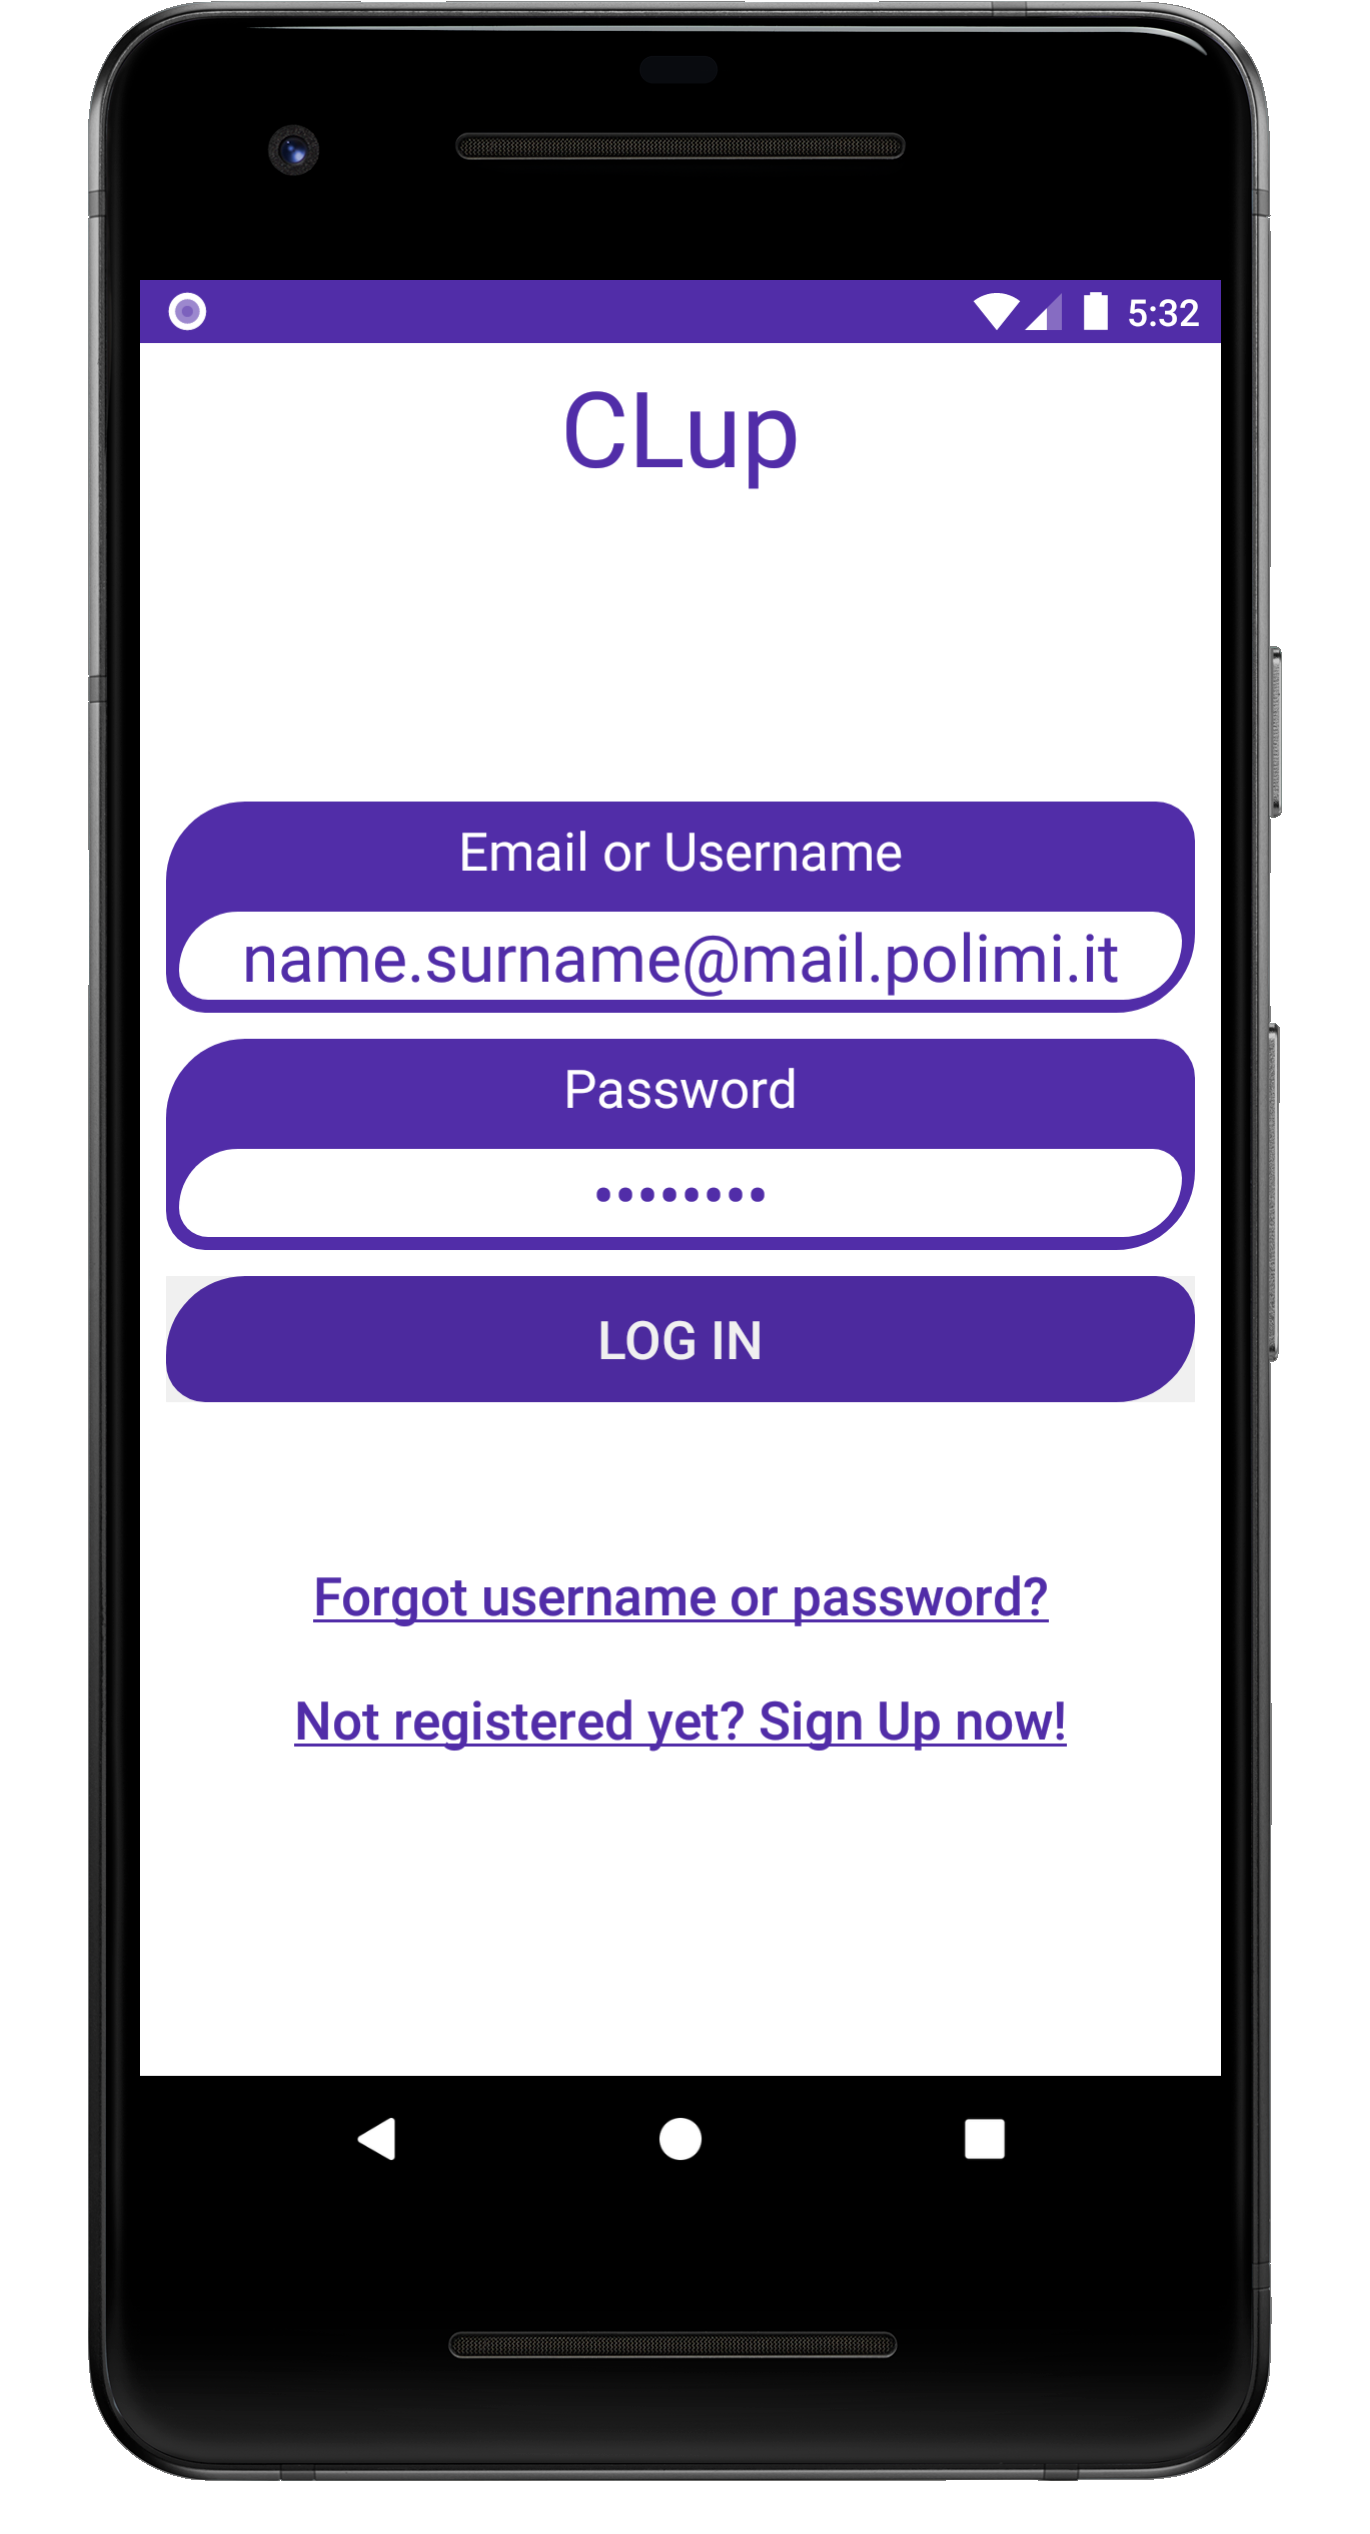
\includegraphics[width=0.4\textwidth]{images/log_in.png}}
	\subfigure[Sign Up page.]{\label{fig:SignUpMockup}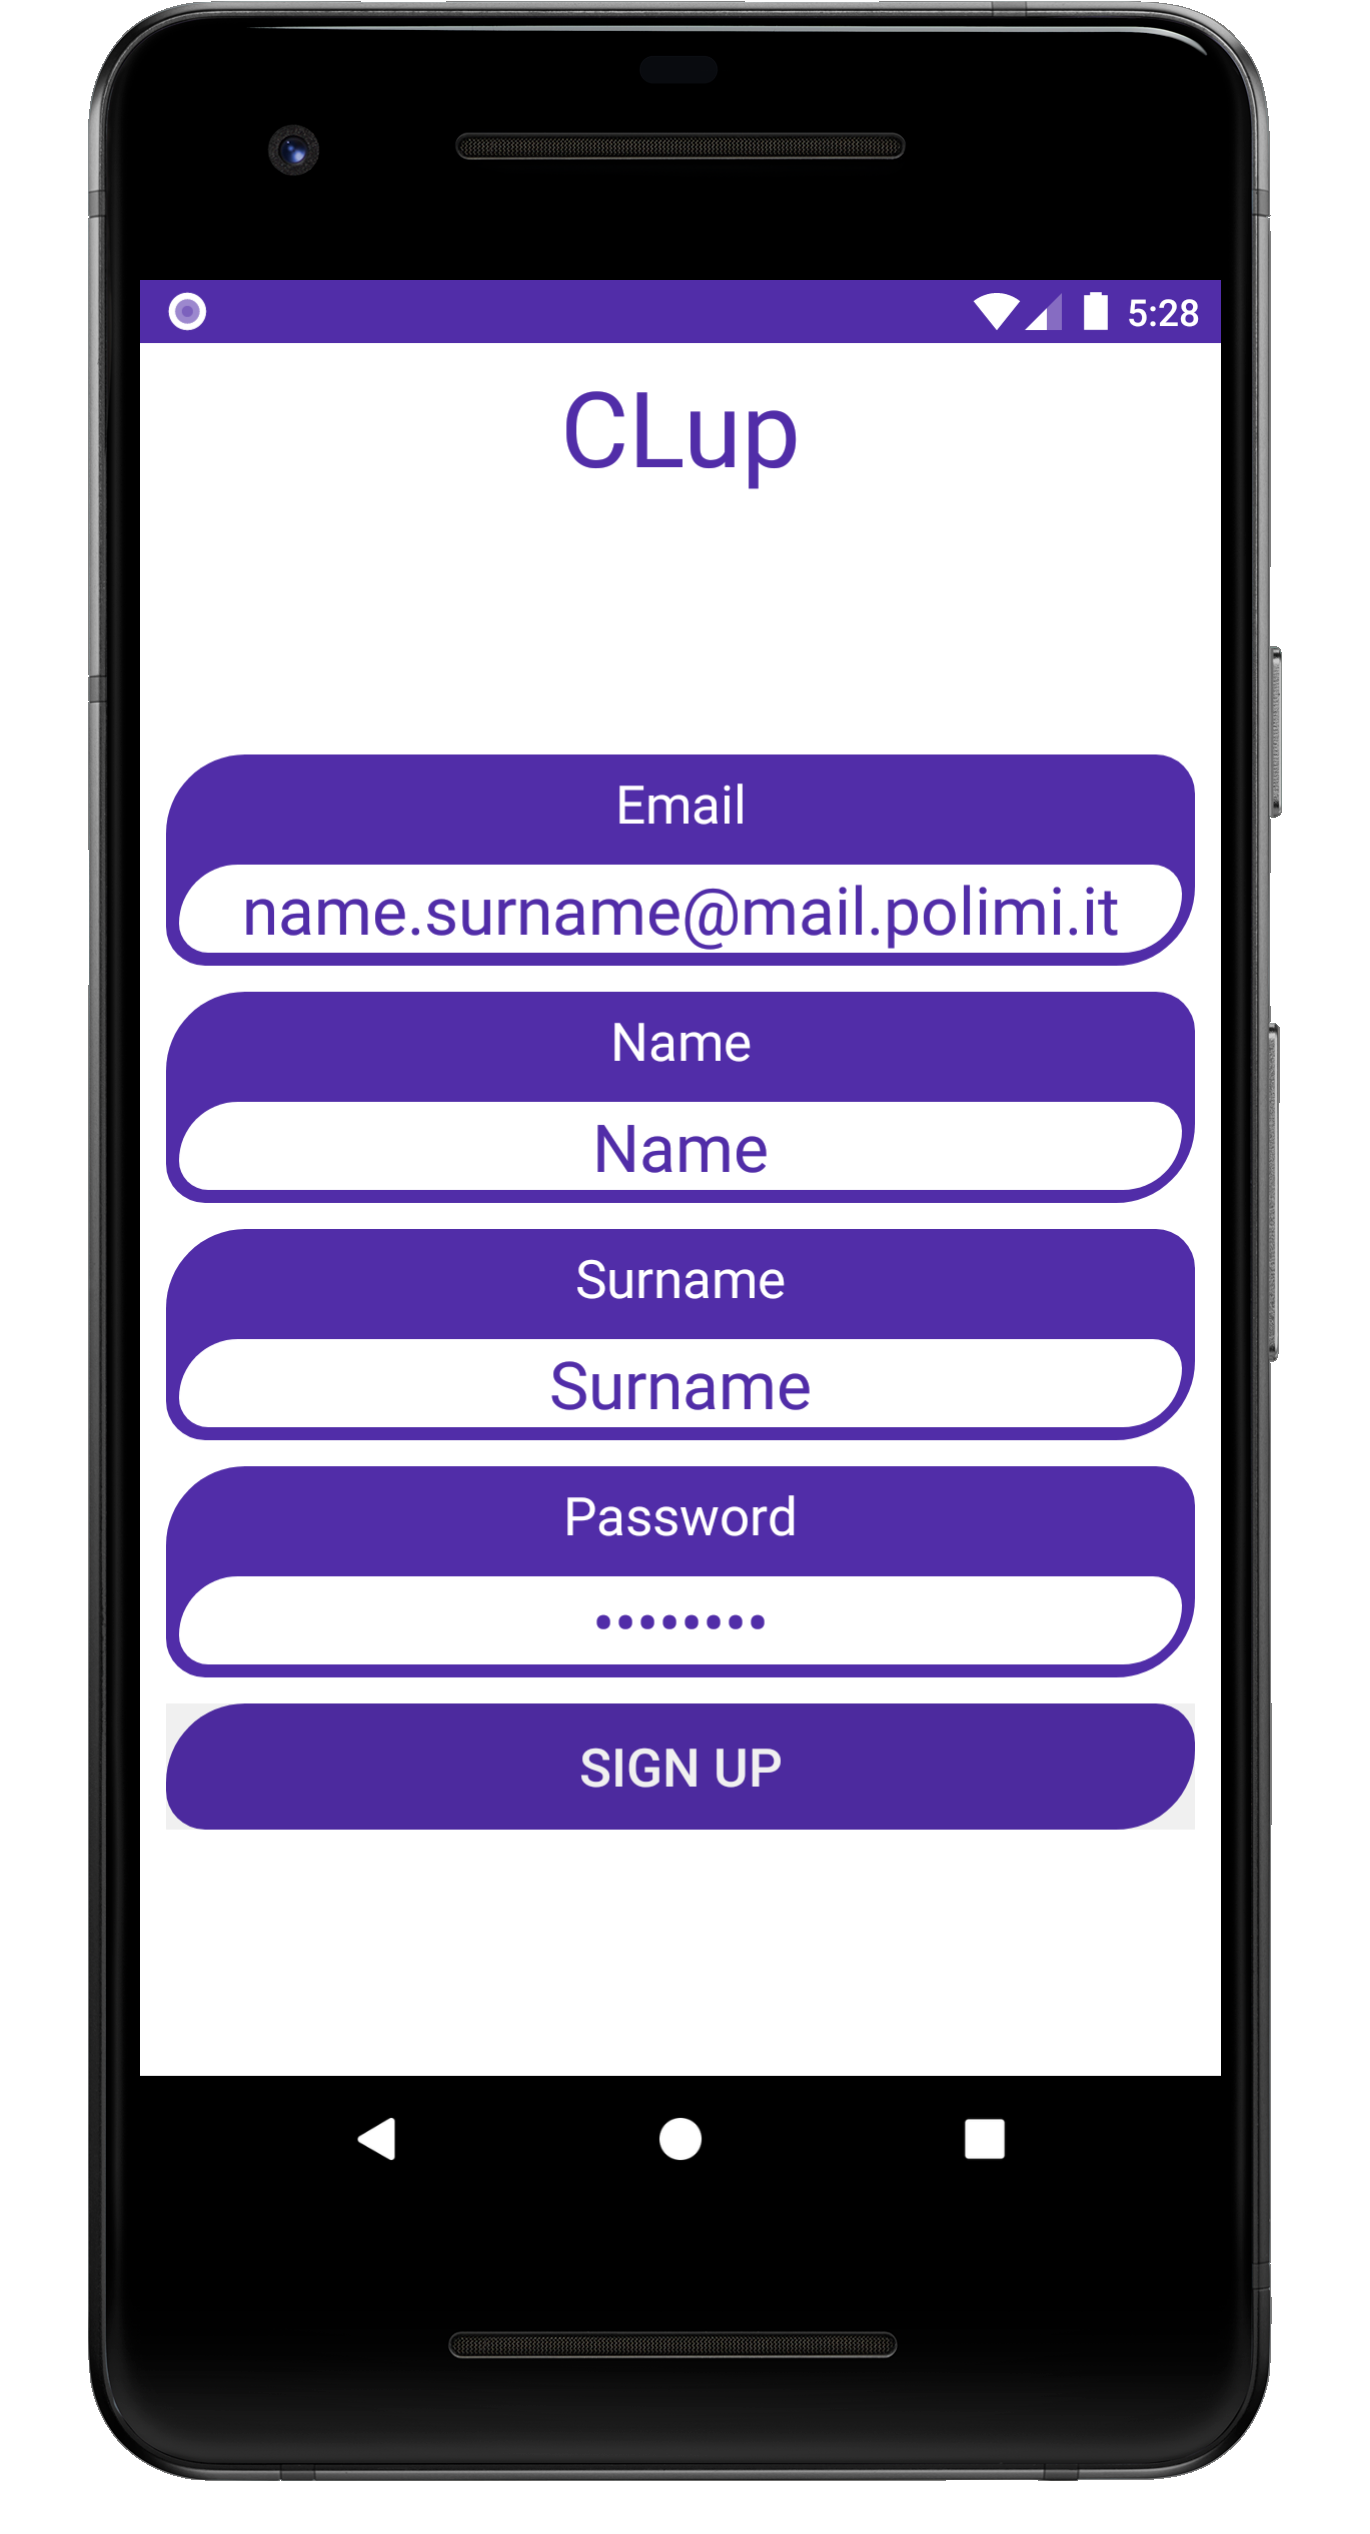
\includegraphics[width=0.4\textwidth]{images/sign_up.png}}
	\caption{Example of Log In and Sign Up pages.}
\end{figure}

Once the login has been completed successfully, the user is redirected to the Home page~\ref{fig:HomeMockup}.
In particular, the reported figure shows the Home page for the customer account with all the functionalities. The application, knowing the type of account, is able to show different buttons. For example, in case of physical spot account, the application will display only the Lining Up button, hiding the others. In case of store manager account, there will be displayed only buttons to control the queue and to analyze the statistics. 

\begin{figure}[H]
	\centering
	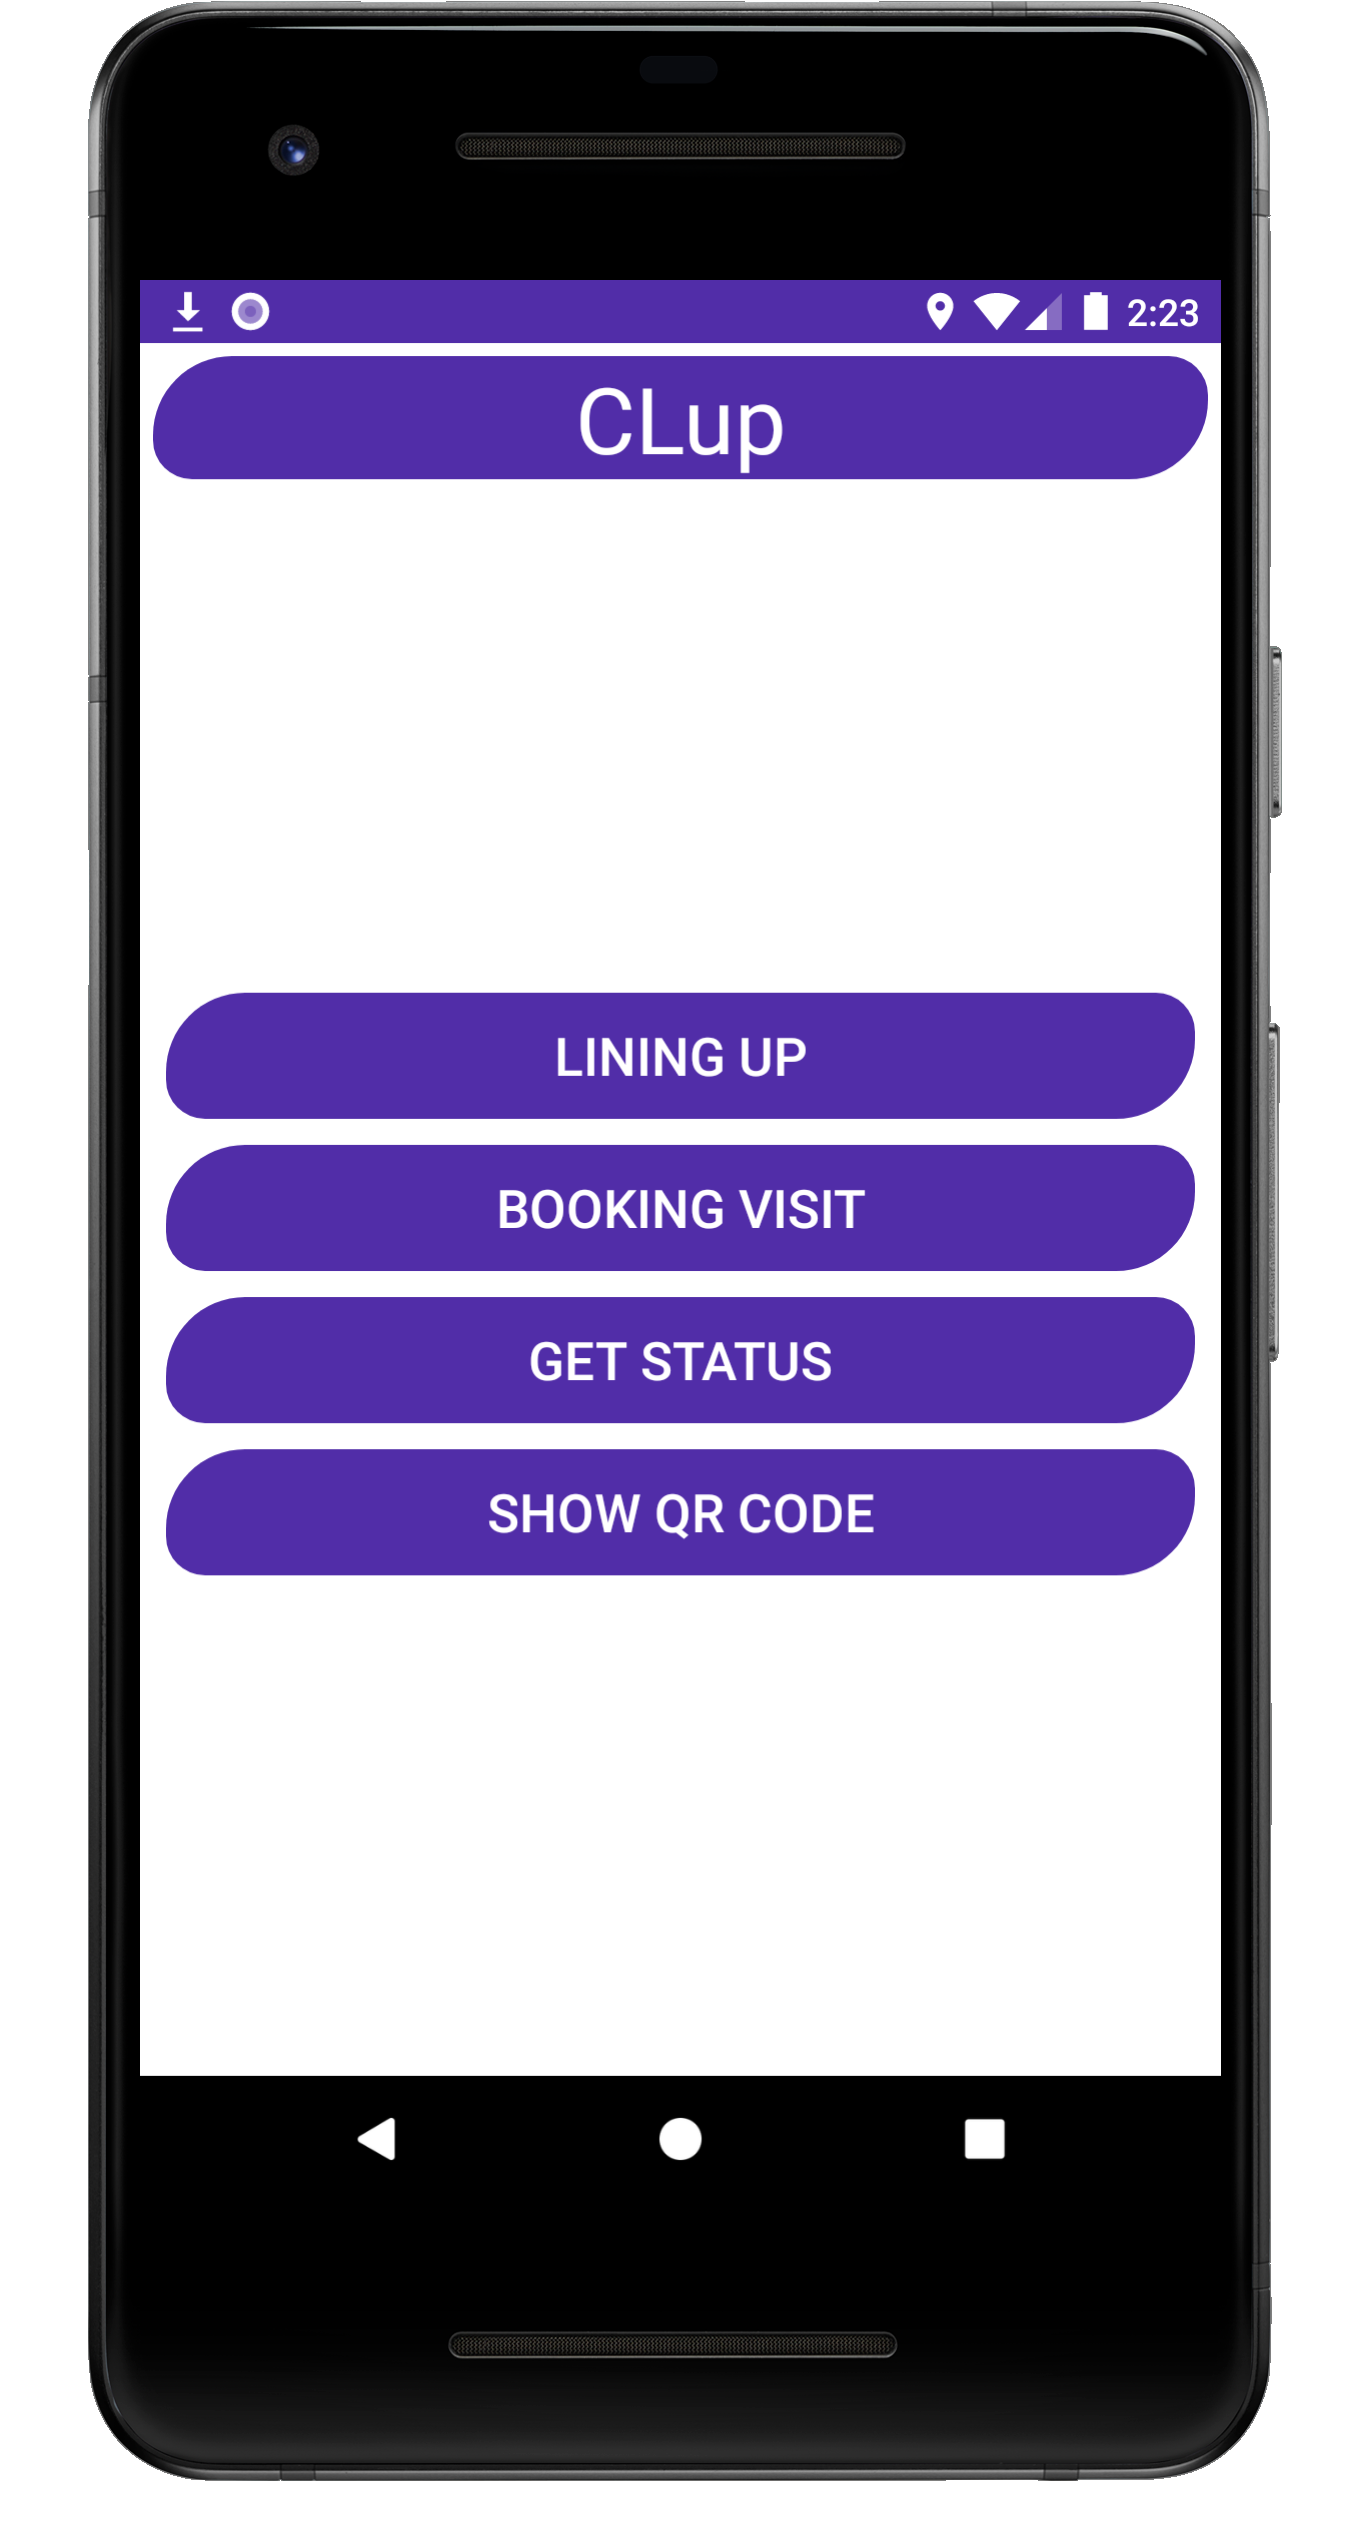
\includegraphics[width=0.35\textwidth]{images/home.png}
	\caption{Home page.}
	\label{fig:HomeMockup}
\end{figure}

If a customer wants to line up, or book a visit, he can click on the corresponding button, in this way the application will show the form to insert the requested parameters~\ref{fig:LiningBookingMockup}.
In the mock-up we show how the user can choose the store, the time slot and, in case of booking, the category of grocery, by expanding the drop down menu.

\begin{figure}[H]
	\centering     %%% not \center
	\subfigure[Lining Up page.]{\label{fig:LiningUpMockup}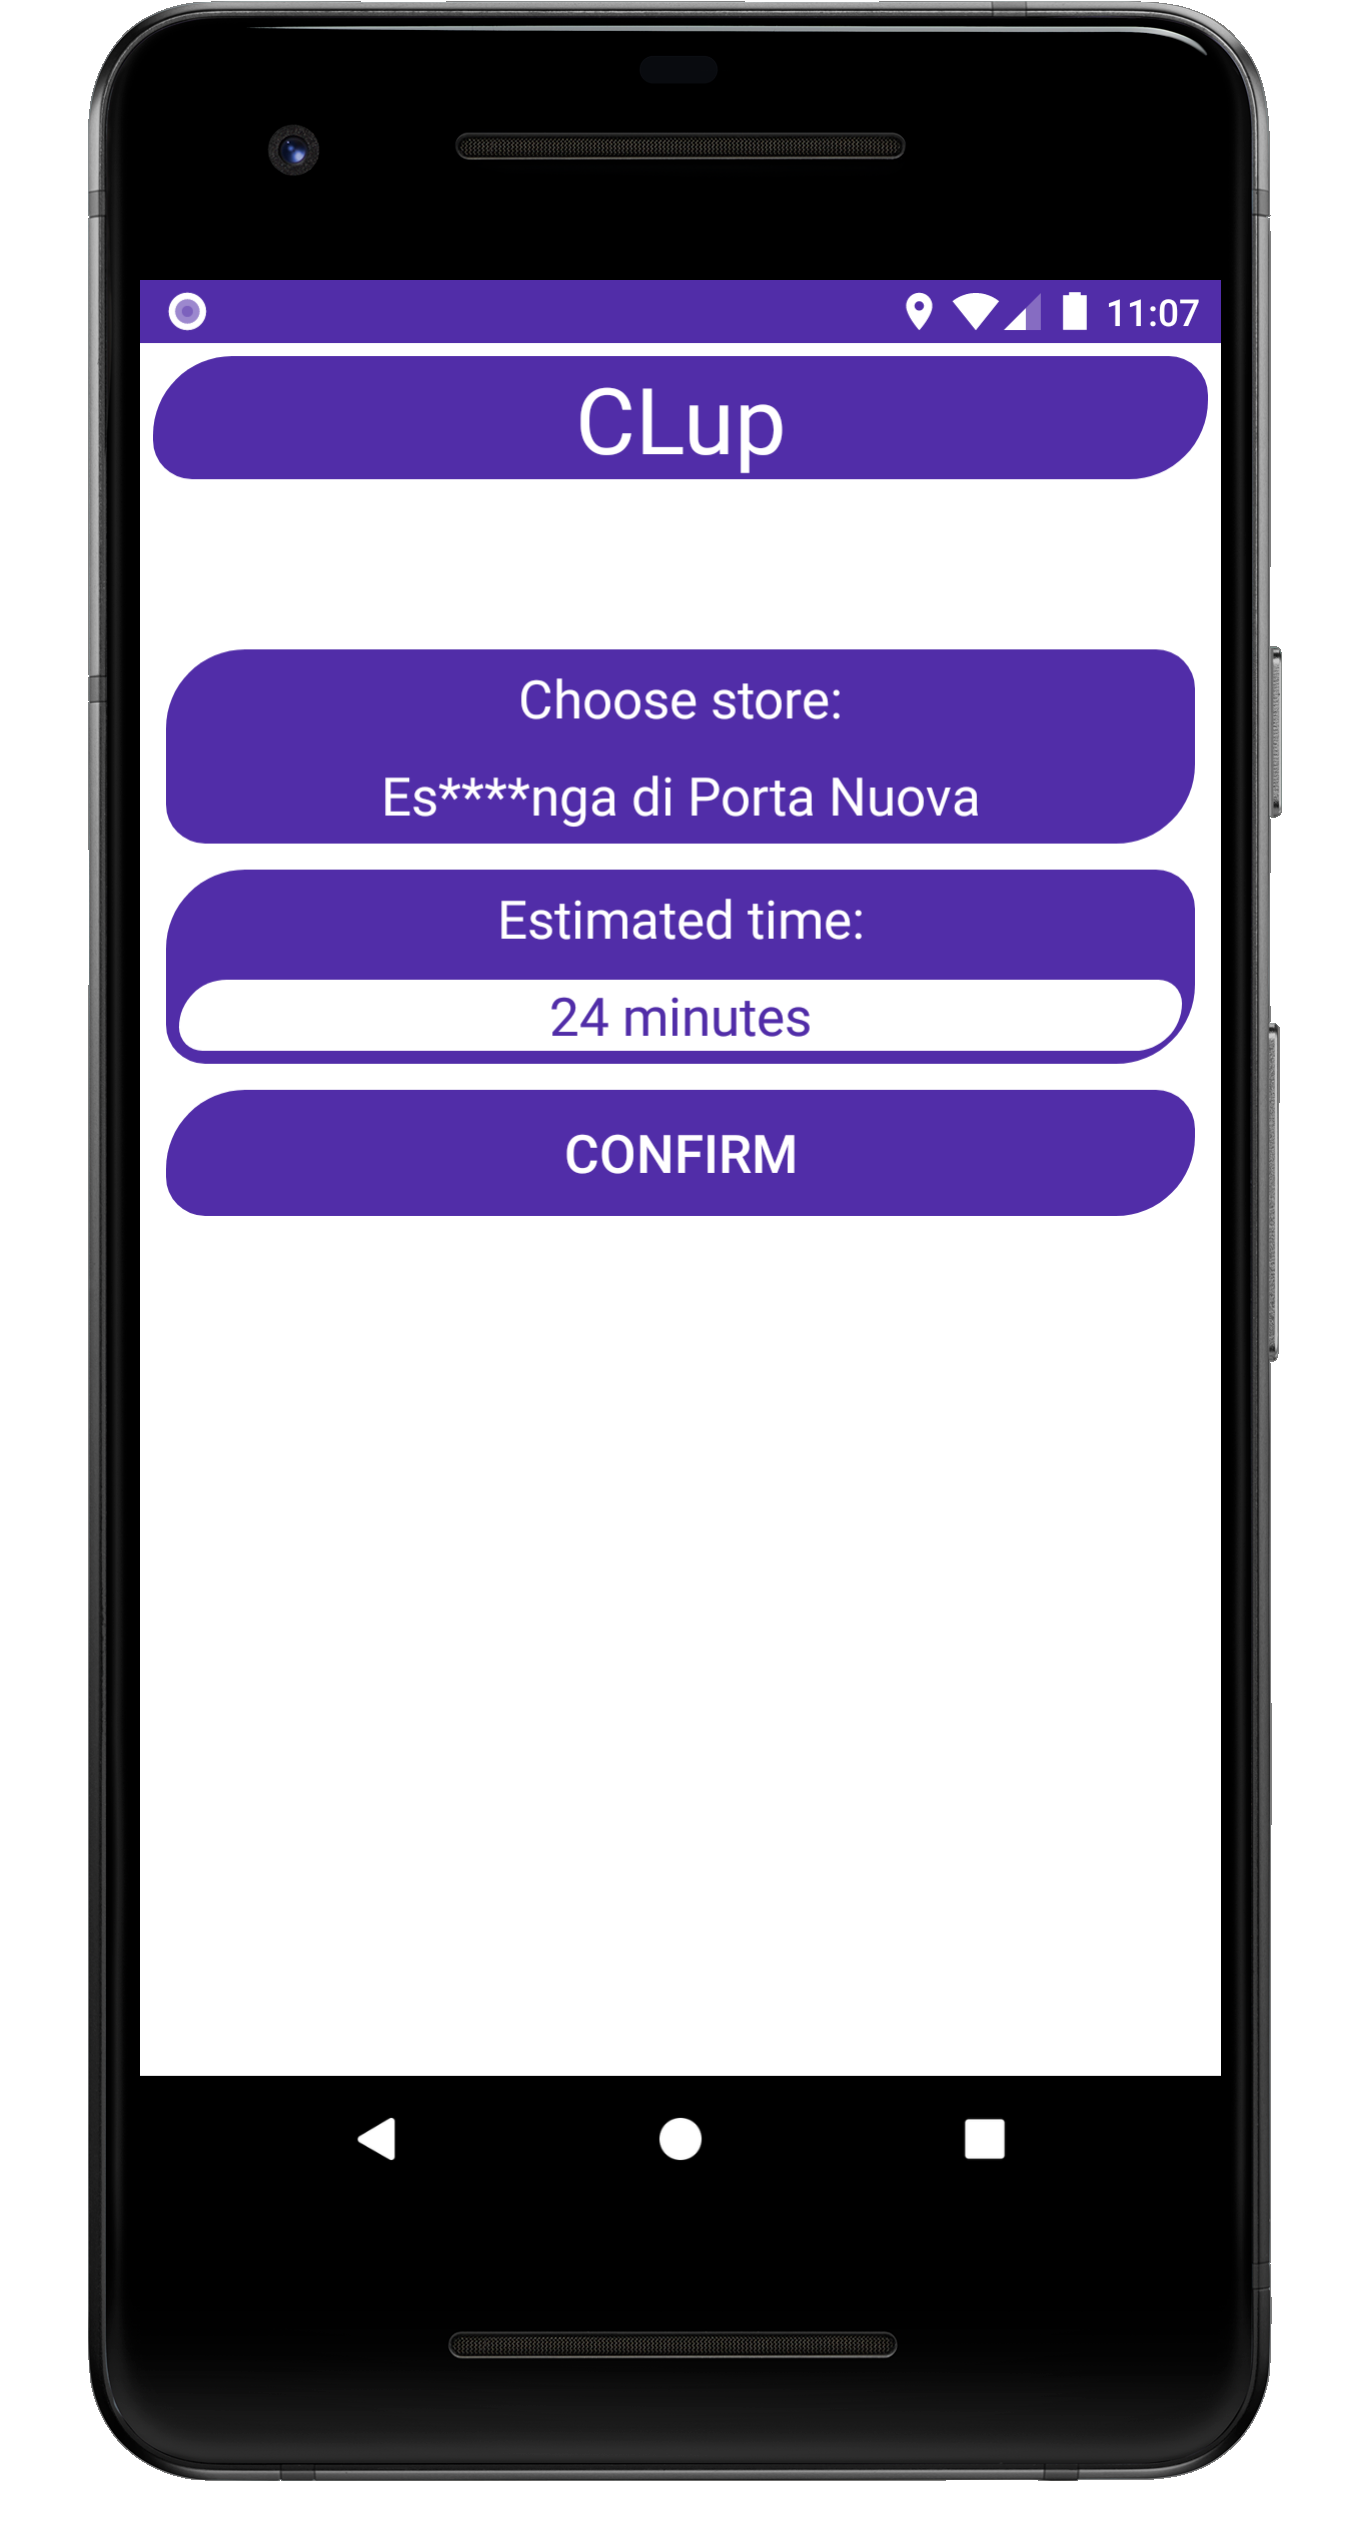
\includegraphics[width=0.4\textwidth]{images/lining_up_01.png}}
	\subfigure[Booking Visit page.]{\label{fig:BookingVisitMockup}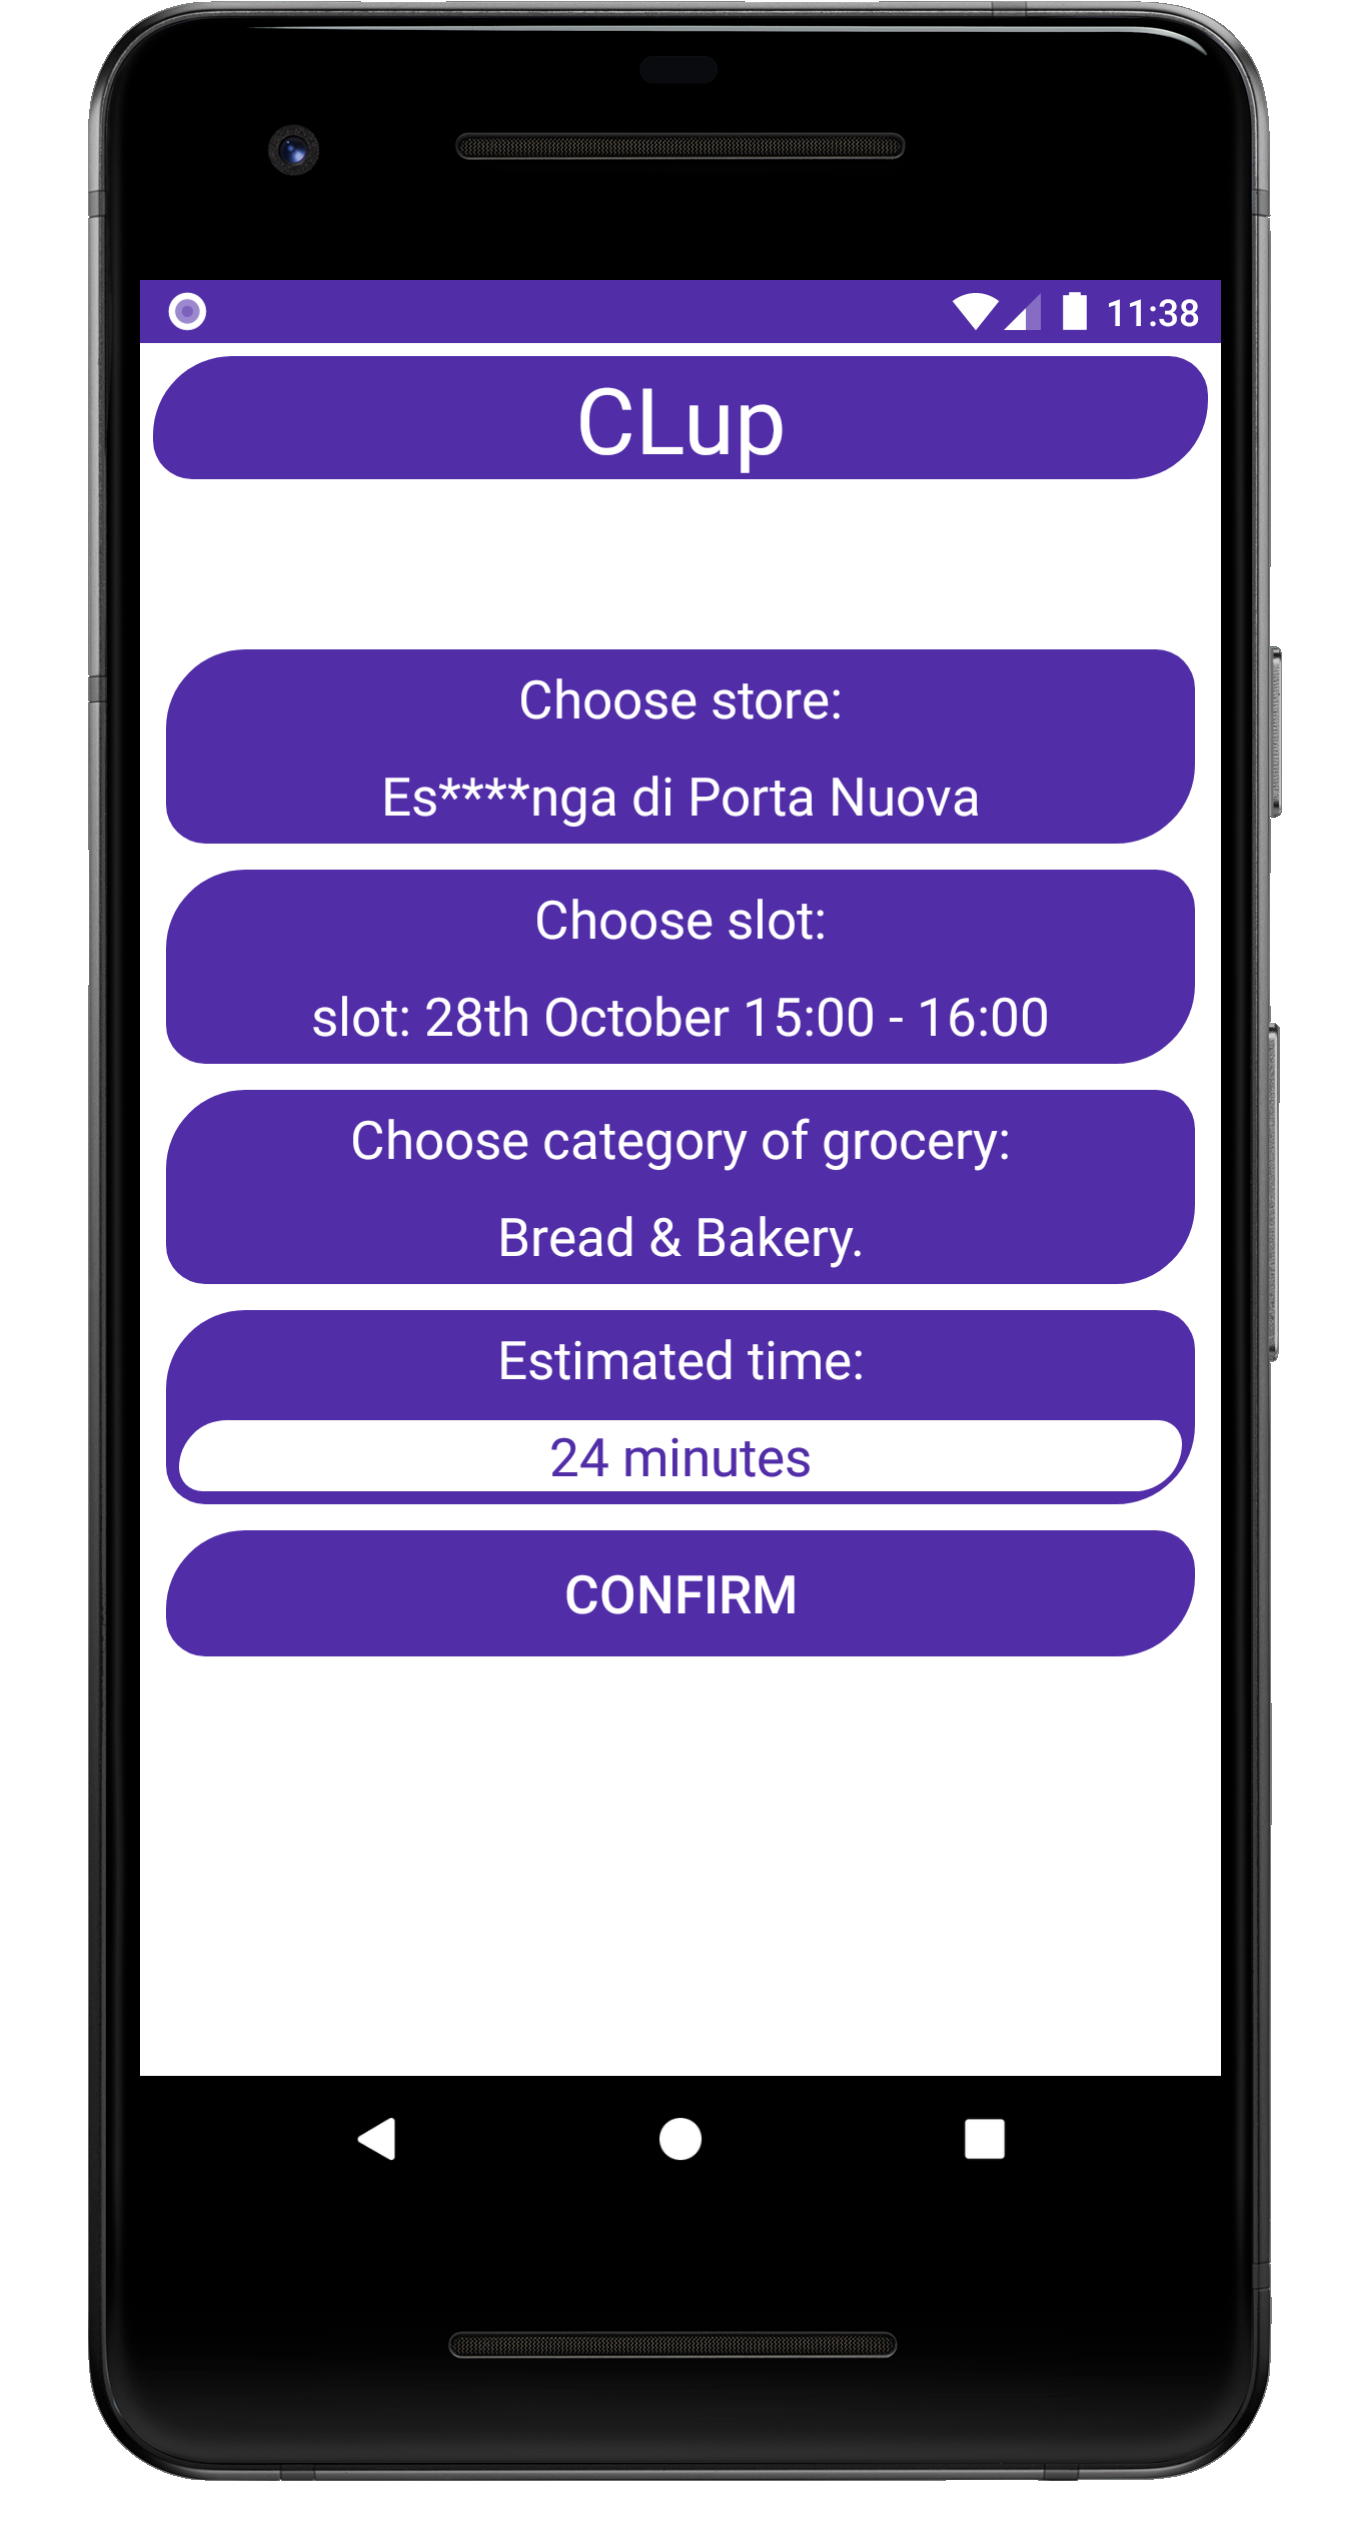
\includegraphics[width=0.4\textwidth]{images/booking_visit_01.png}}
	
	\subfigure[Lining Up page with expanded spinner.]{\label{fig:LiningUp2Mockup}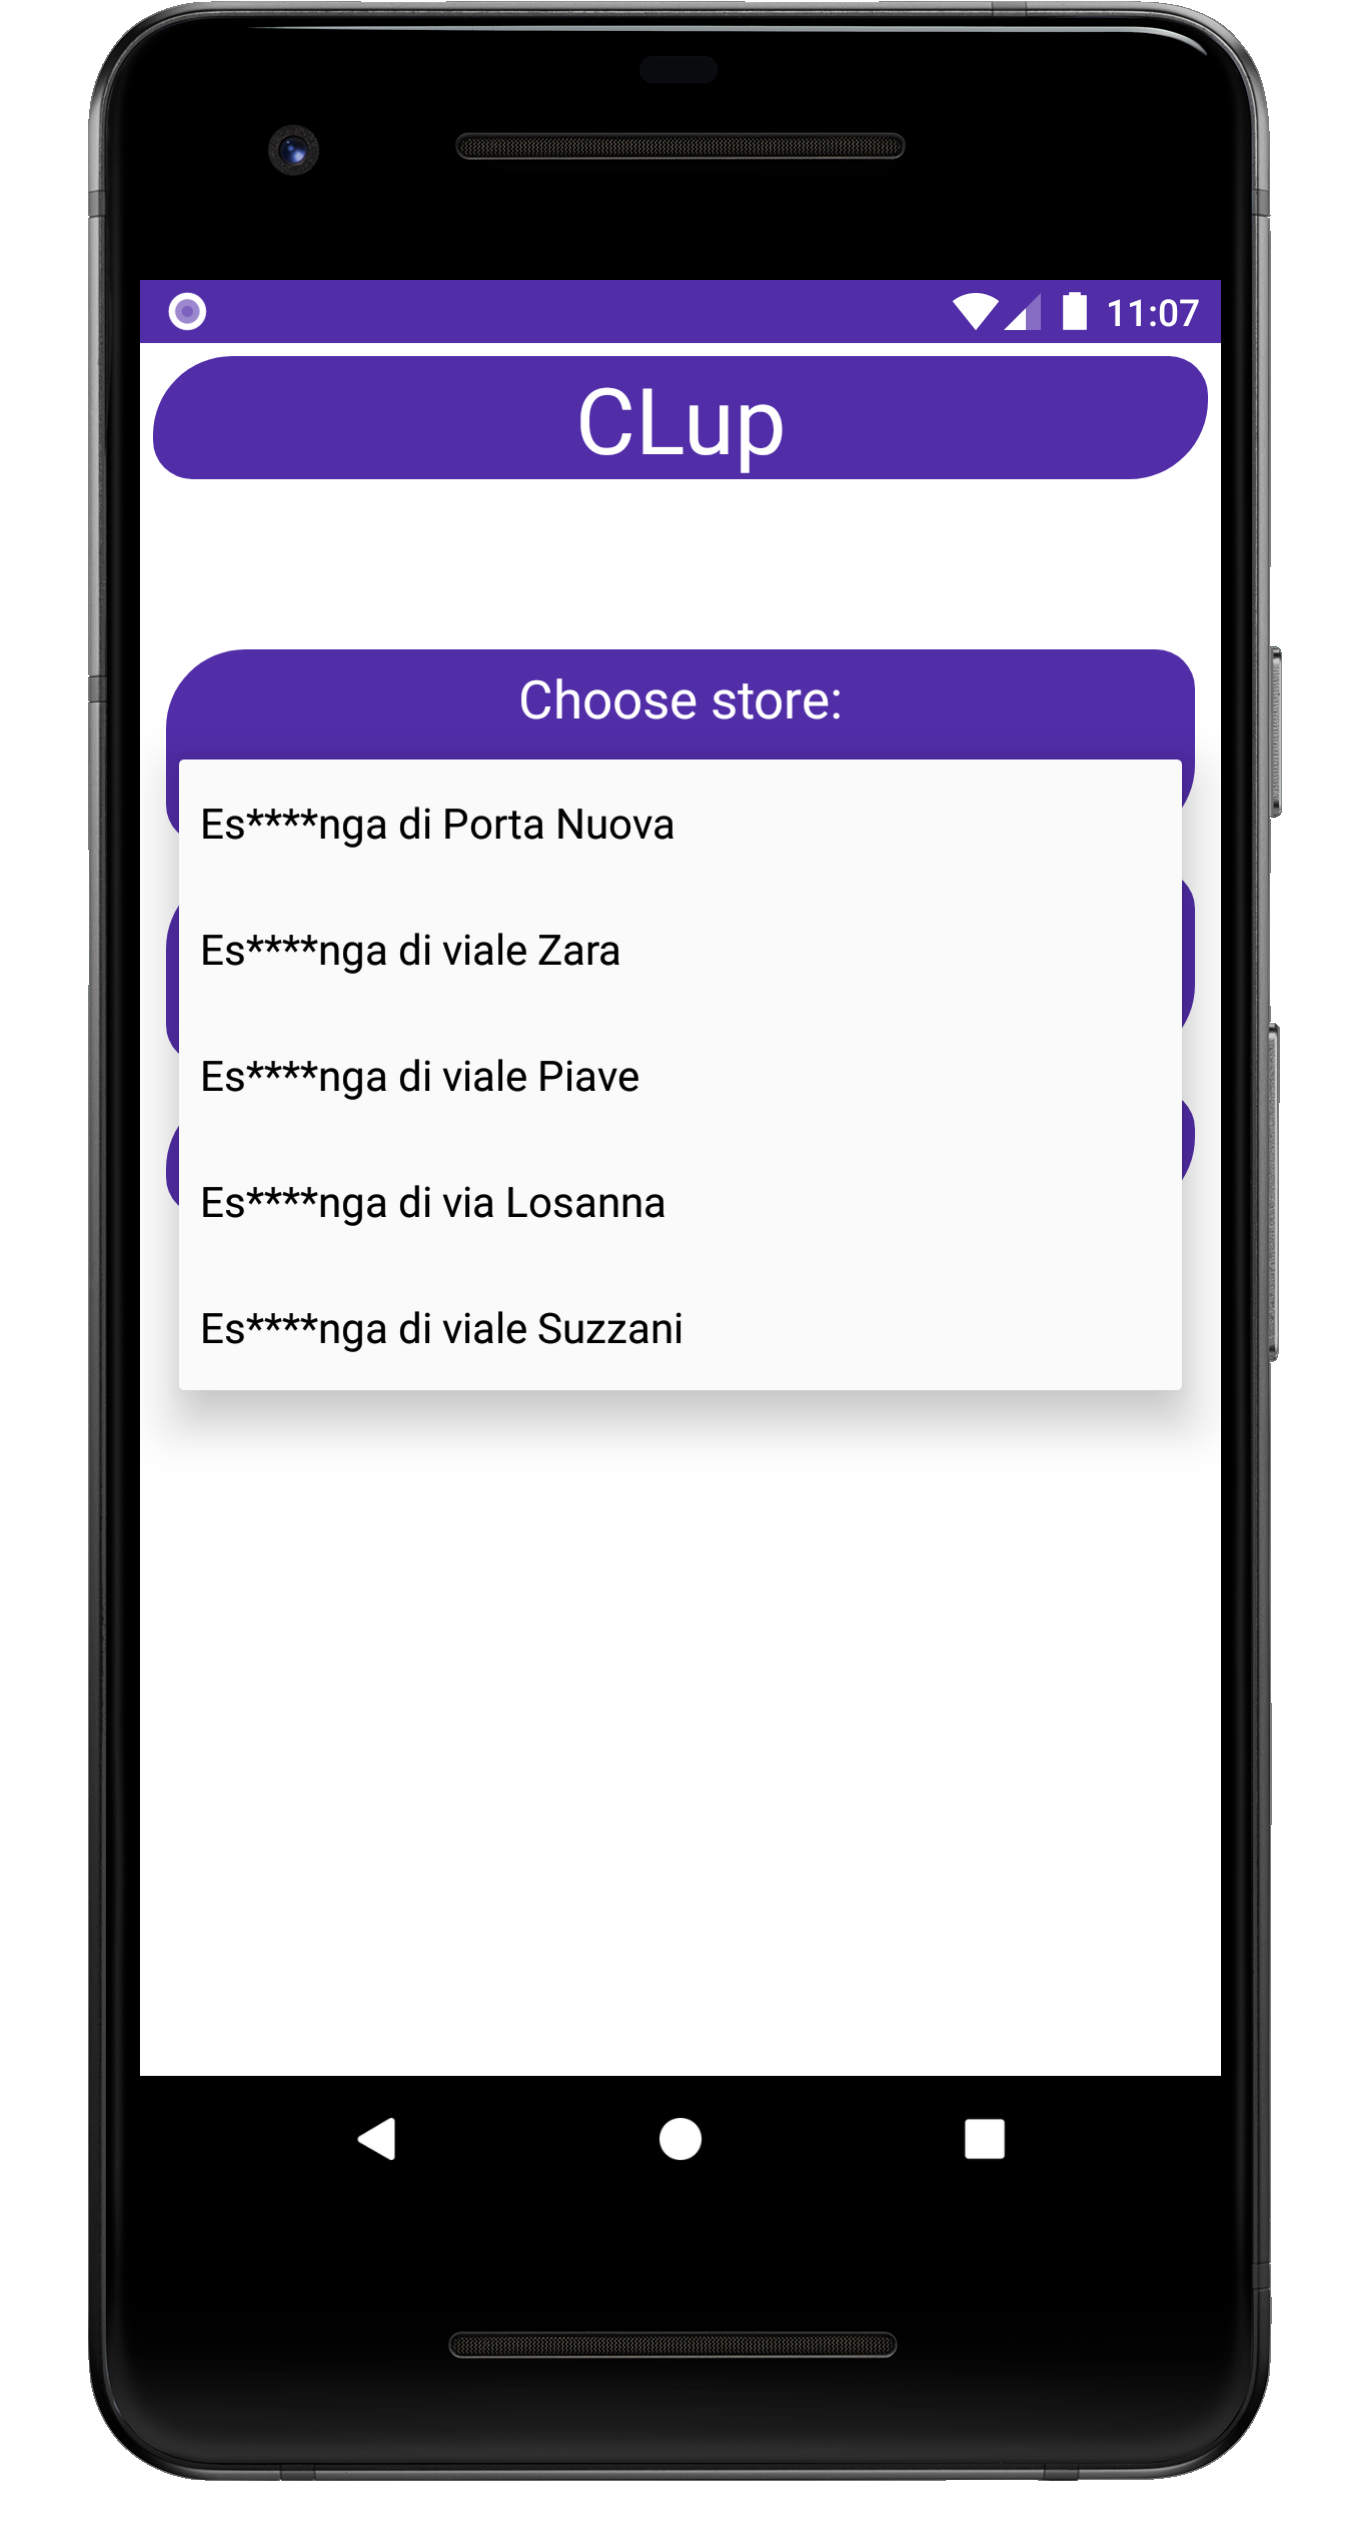
\includegraphics[width=0.4\textwidth]{images/lining_up_02.png}}
	\subfigure[Booking Visit page with expanded spinner.]{\label{fig:BookingVisit2Mockup}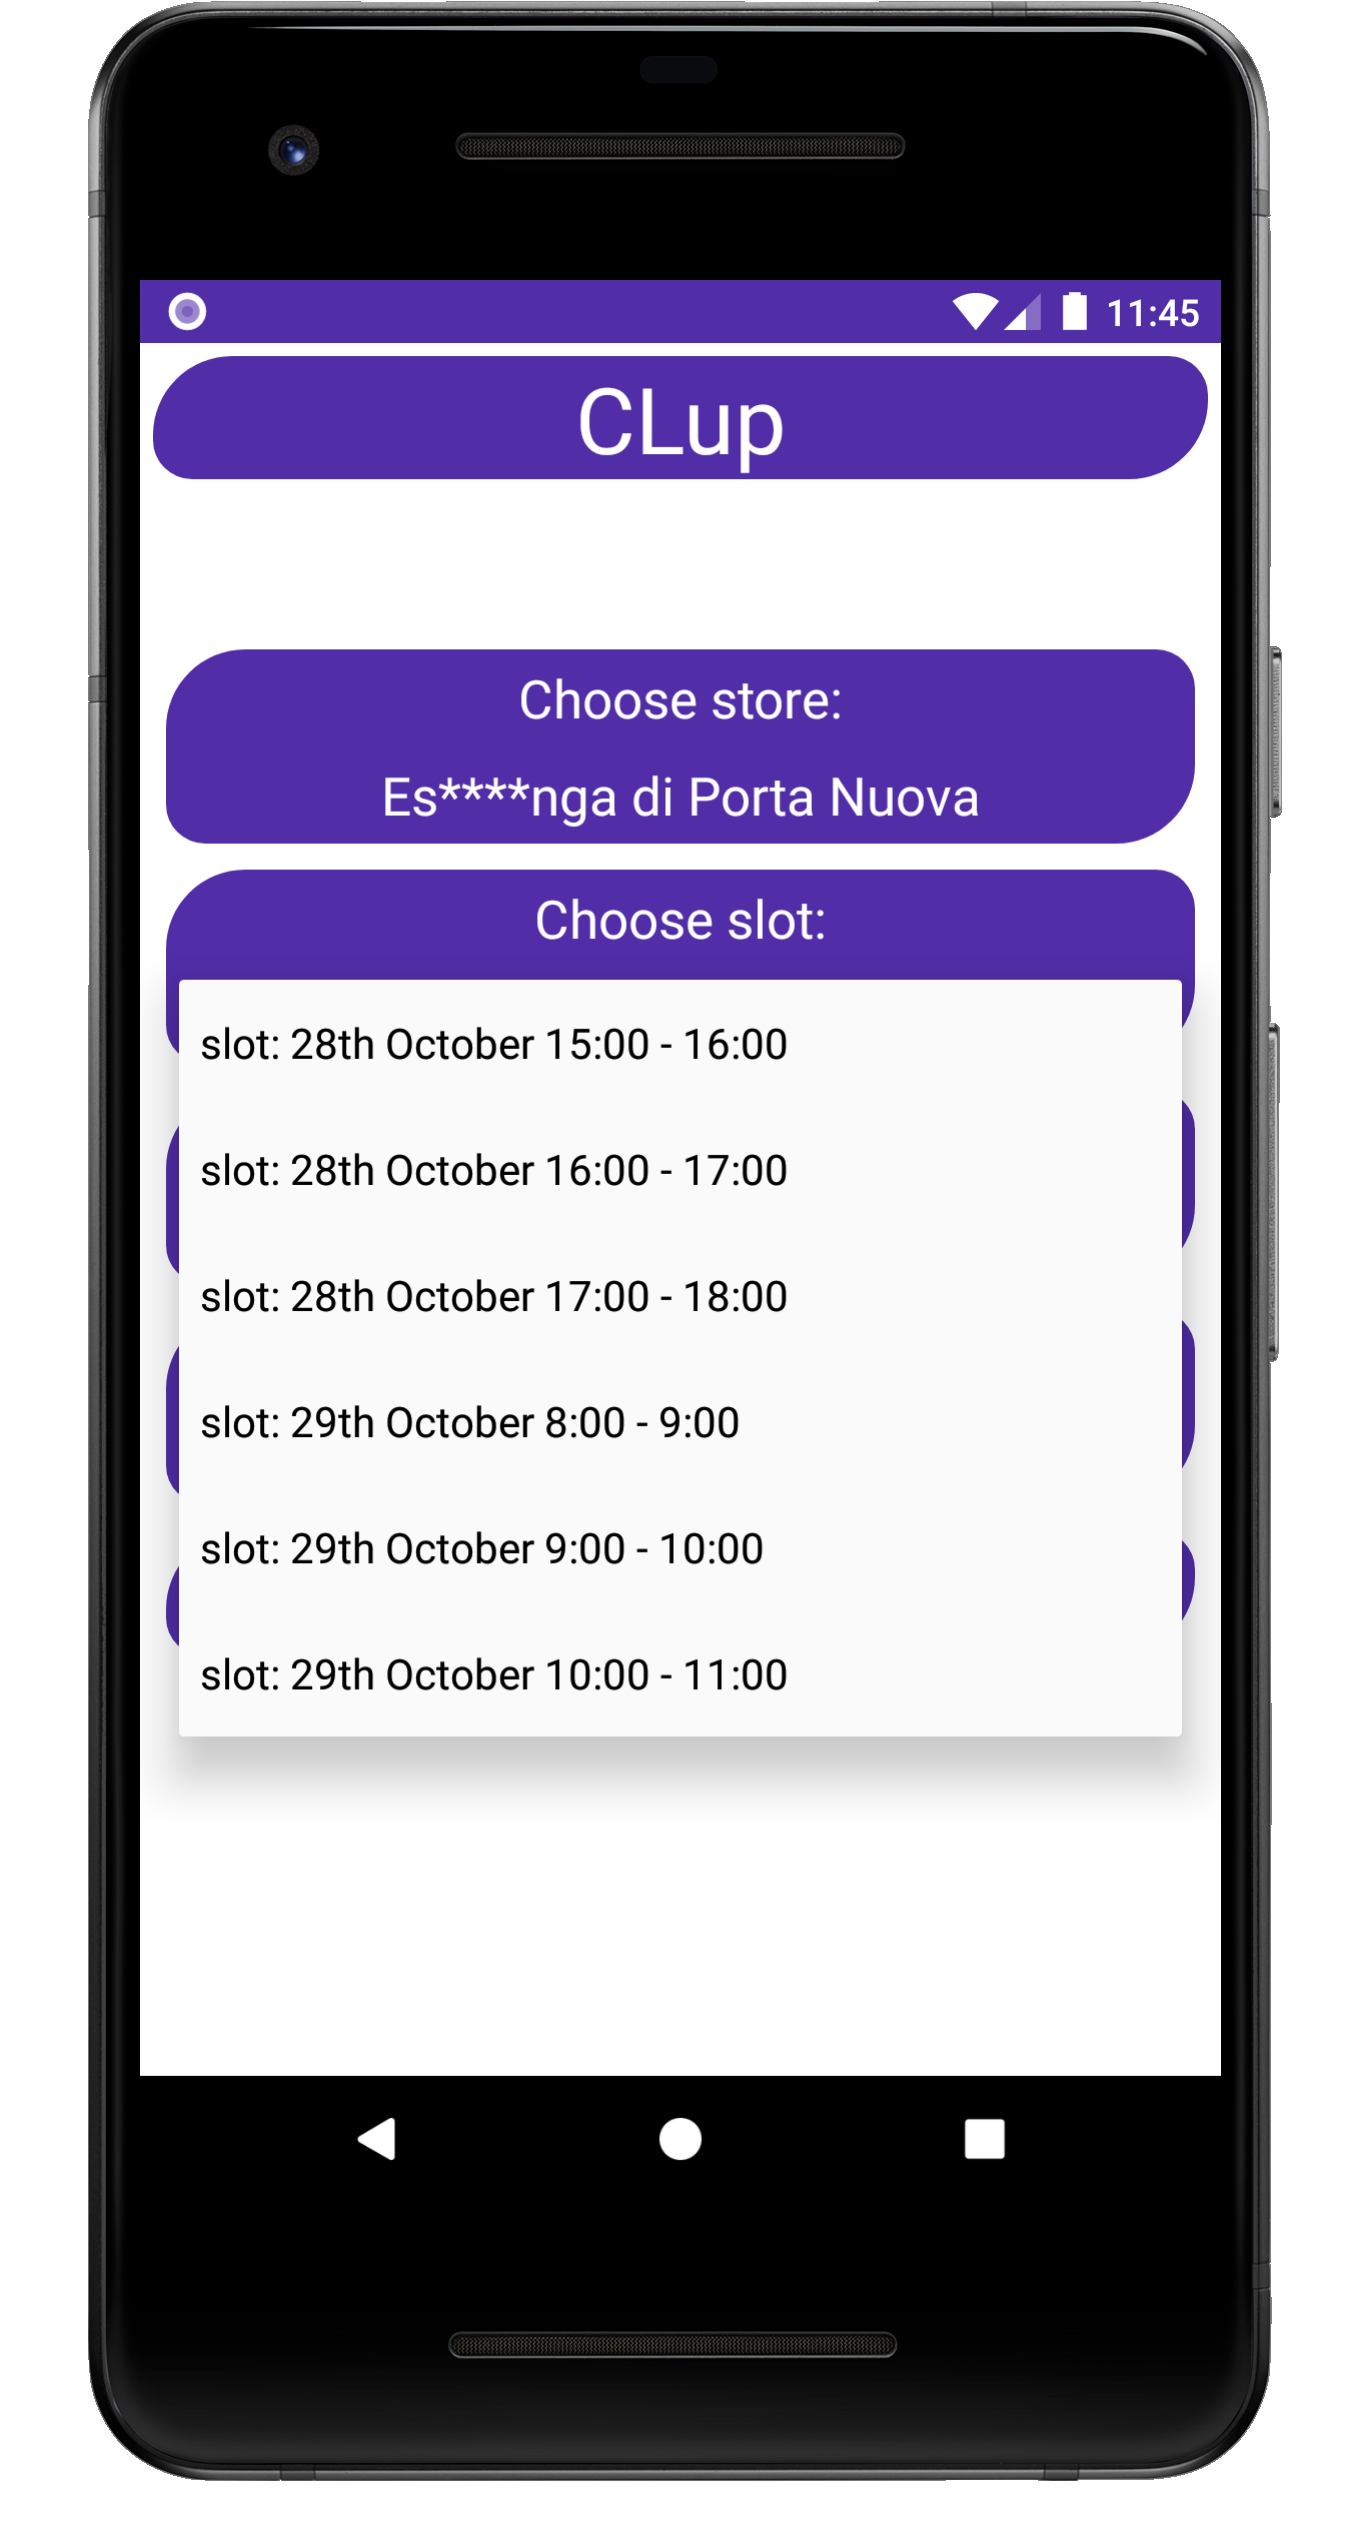
\includegraphics[width=0.4\textwidth]{images/booking_visit_02.png}}
	\caption{Example of Lining Up and Booking Visit pages.}
	\label{fig:LiningBookingMockup}
\end{figure}

The application provides the possibility to check the queue status by clicking on the Get Status button and to watch the QR code by clicking on the relative button.
These buttons aren't visible from the Home page until the user performs a lining up, or booking a visit, operation.
If visible, the users will be able to see the interfaces: \ref{fig:GetStatusMockup}, \ref{fig:ShowQRMockup}.

\begin{figure}[H]
	\centering     %%% not \center
	\subfigure[Get Status page.]{\label{fig:GetStatusMockup}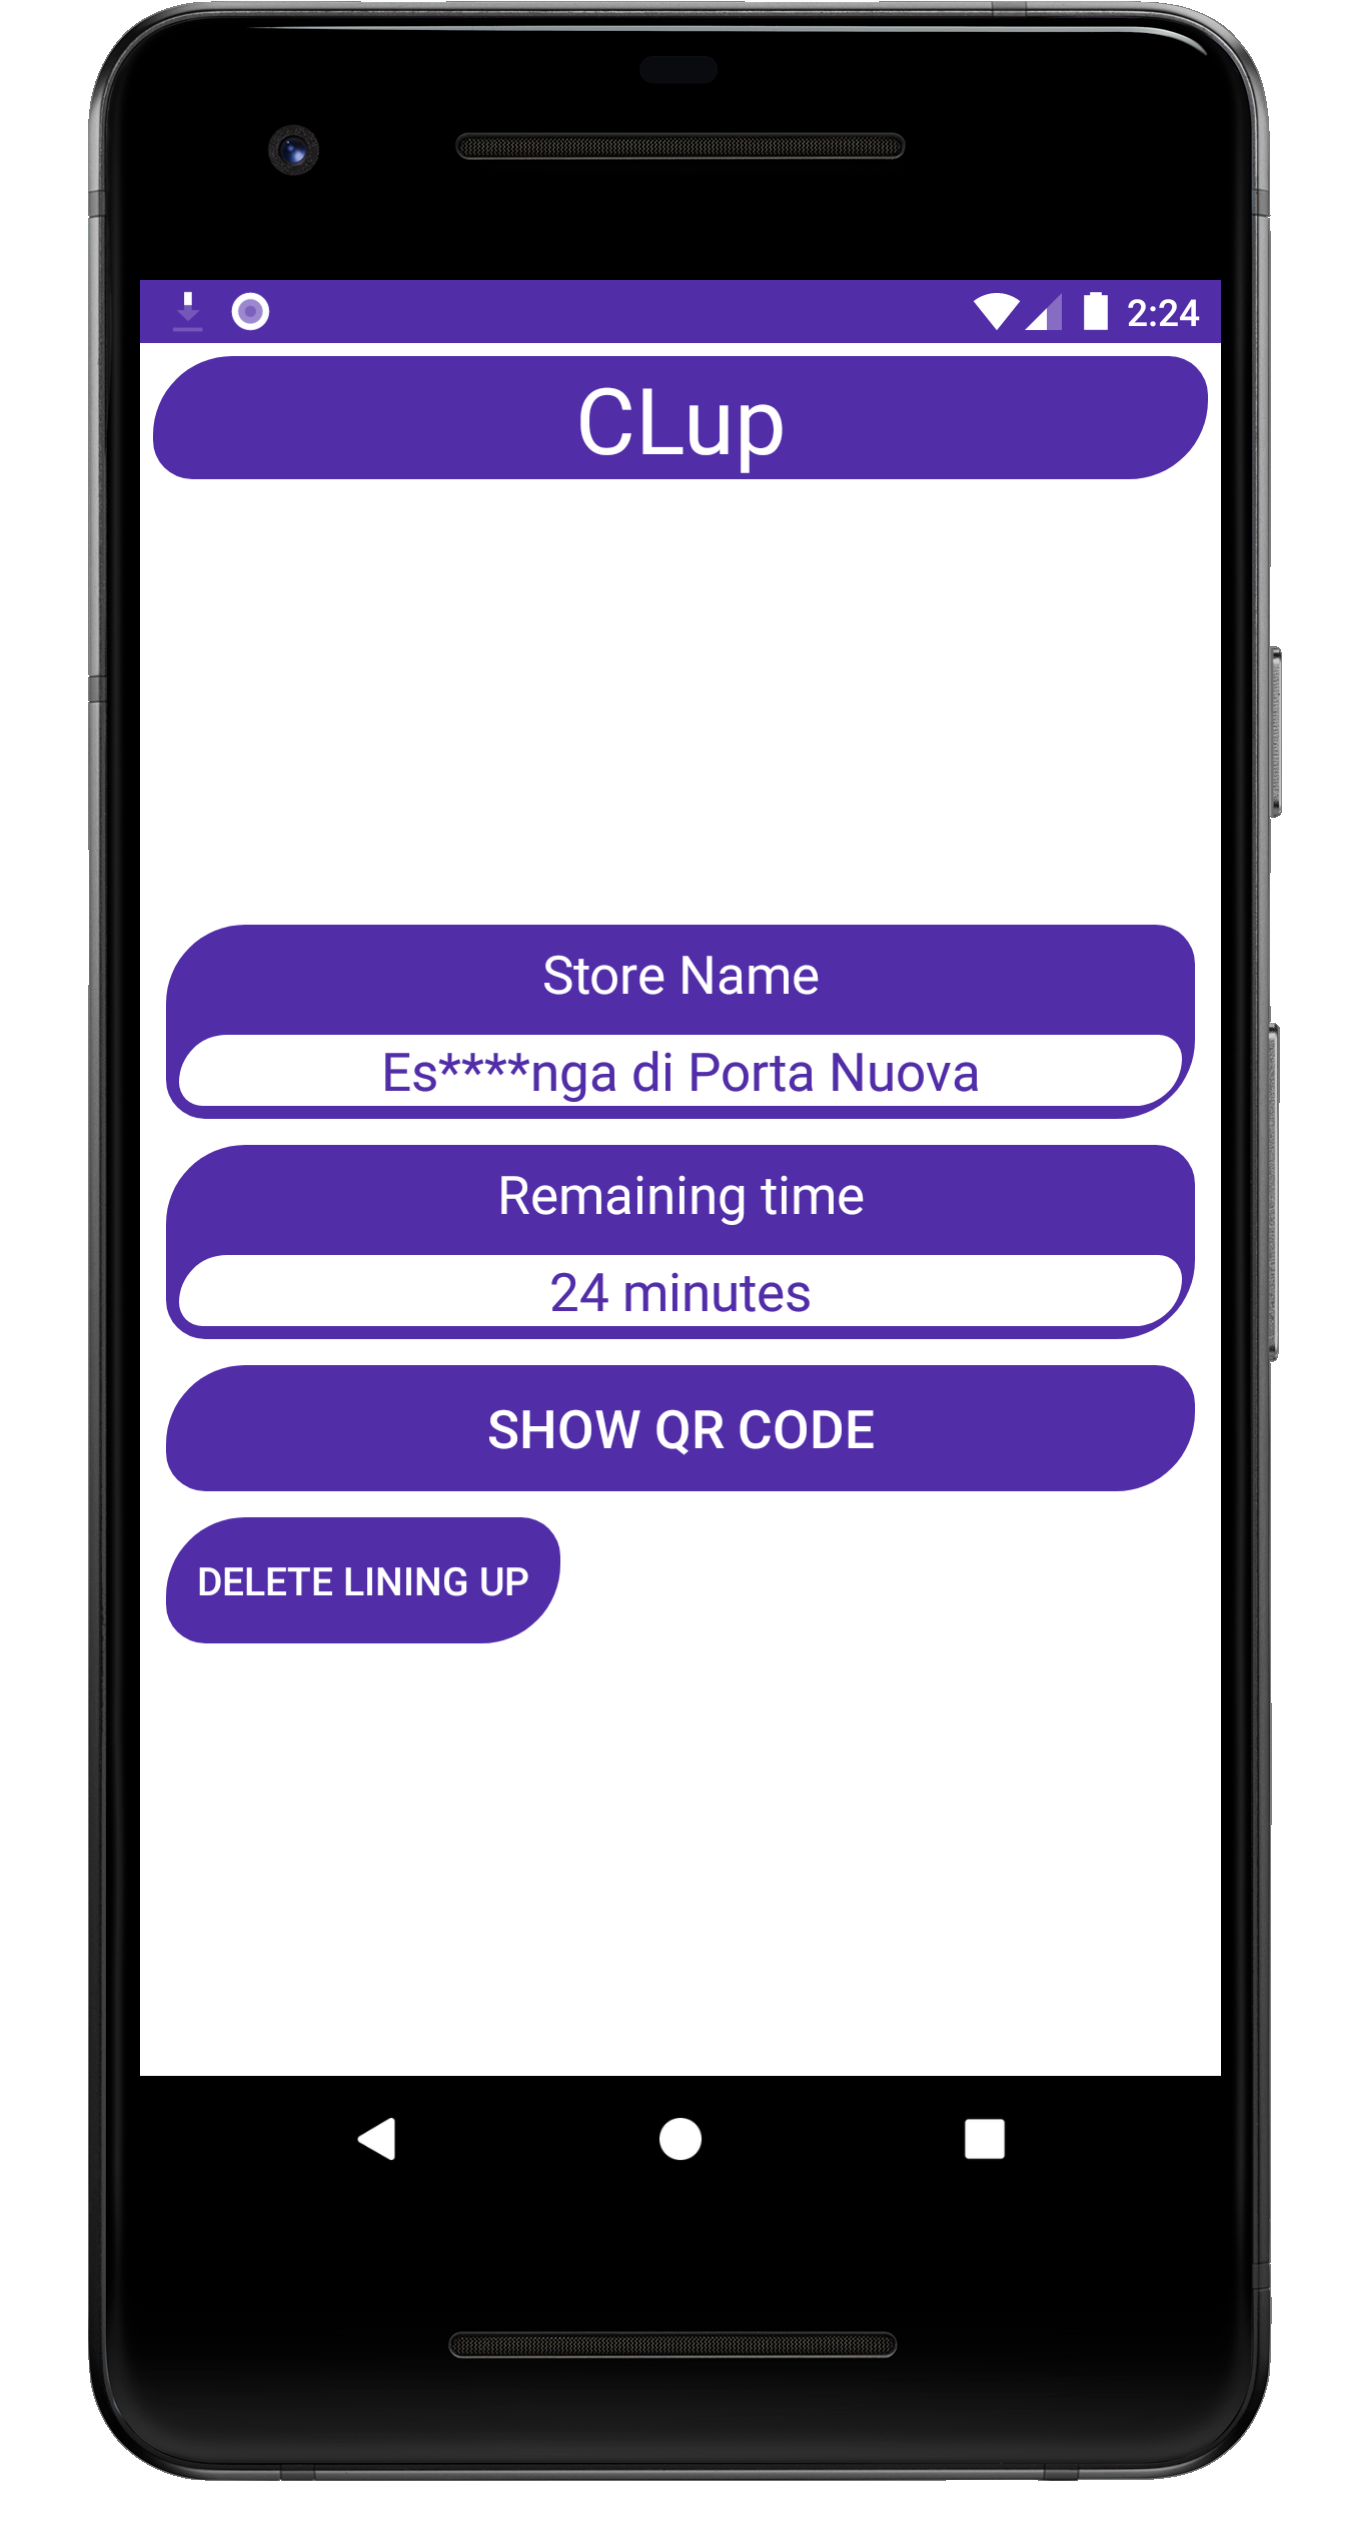
\includegraphics[width=0.4\textwidth]{images/get_status.png}}
	\subfigure[Show QR code page.]{\label{fig:ShowQRMockup}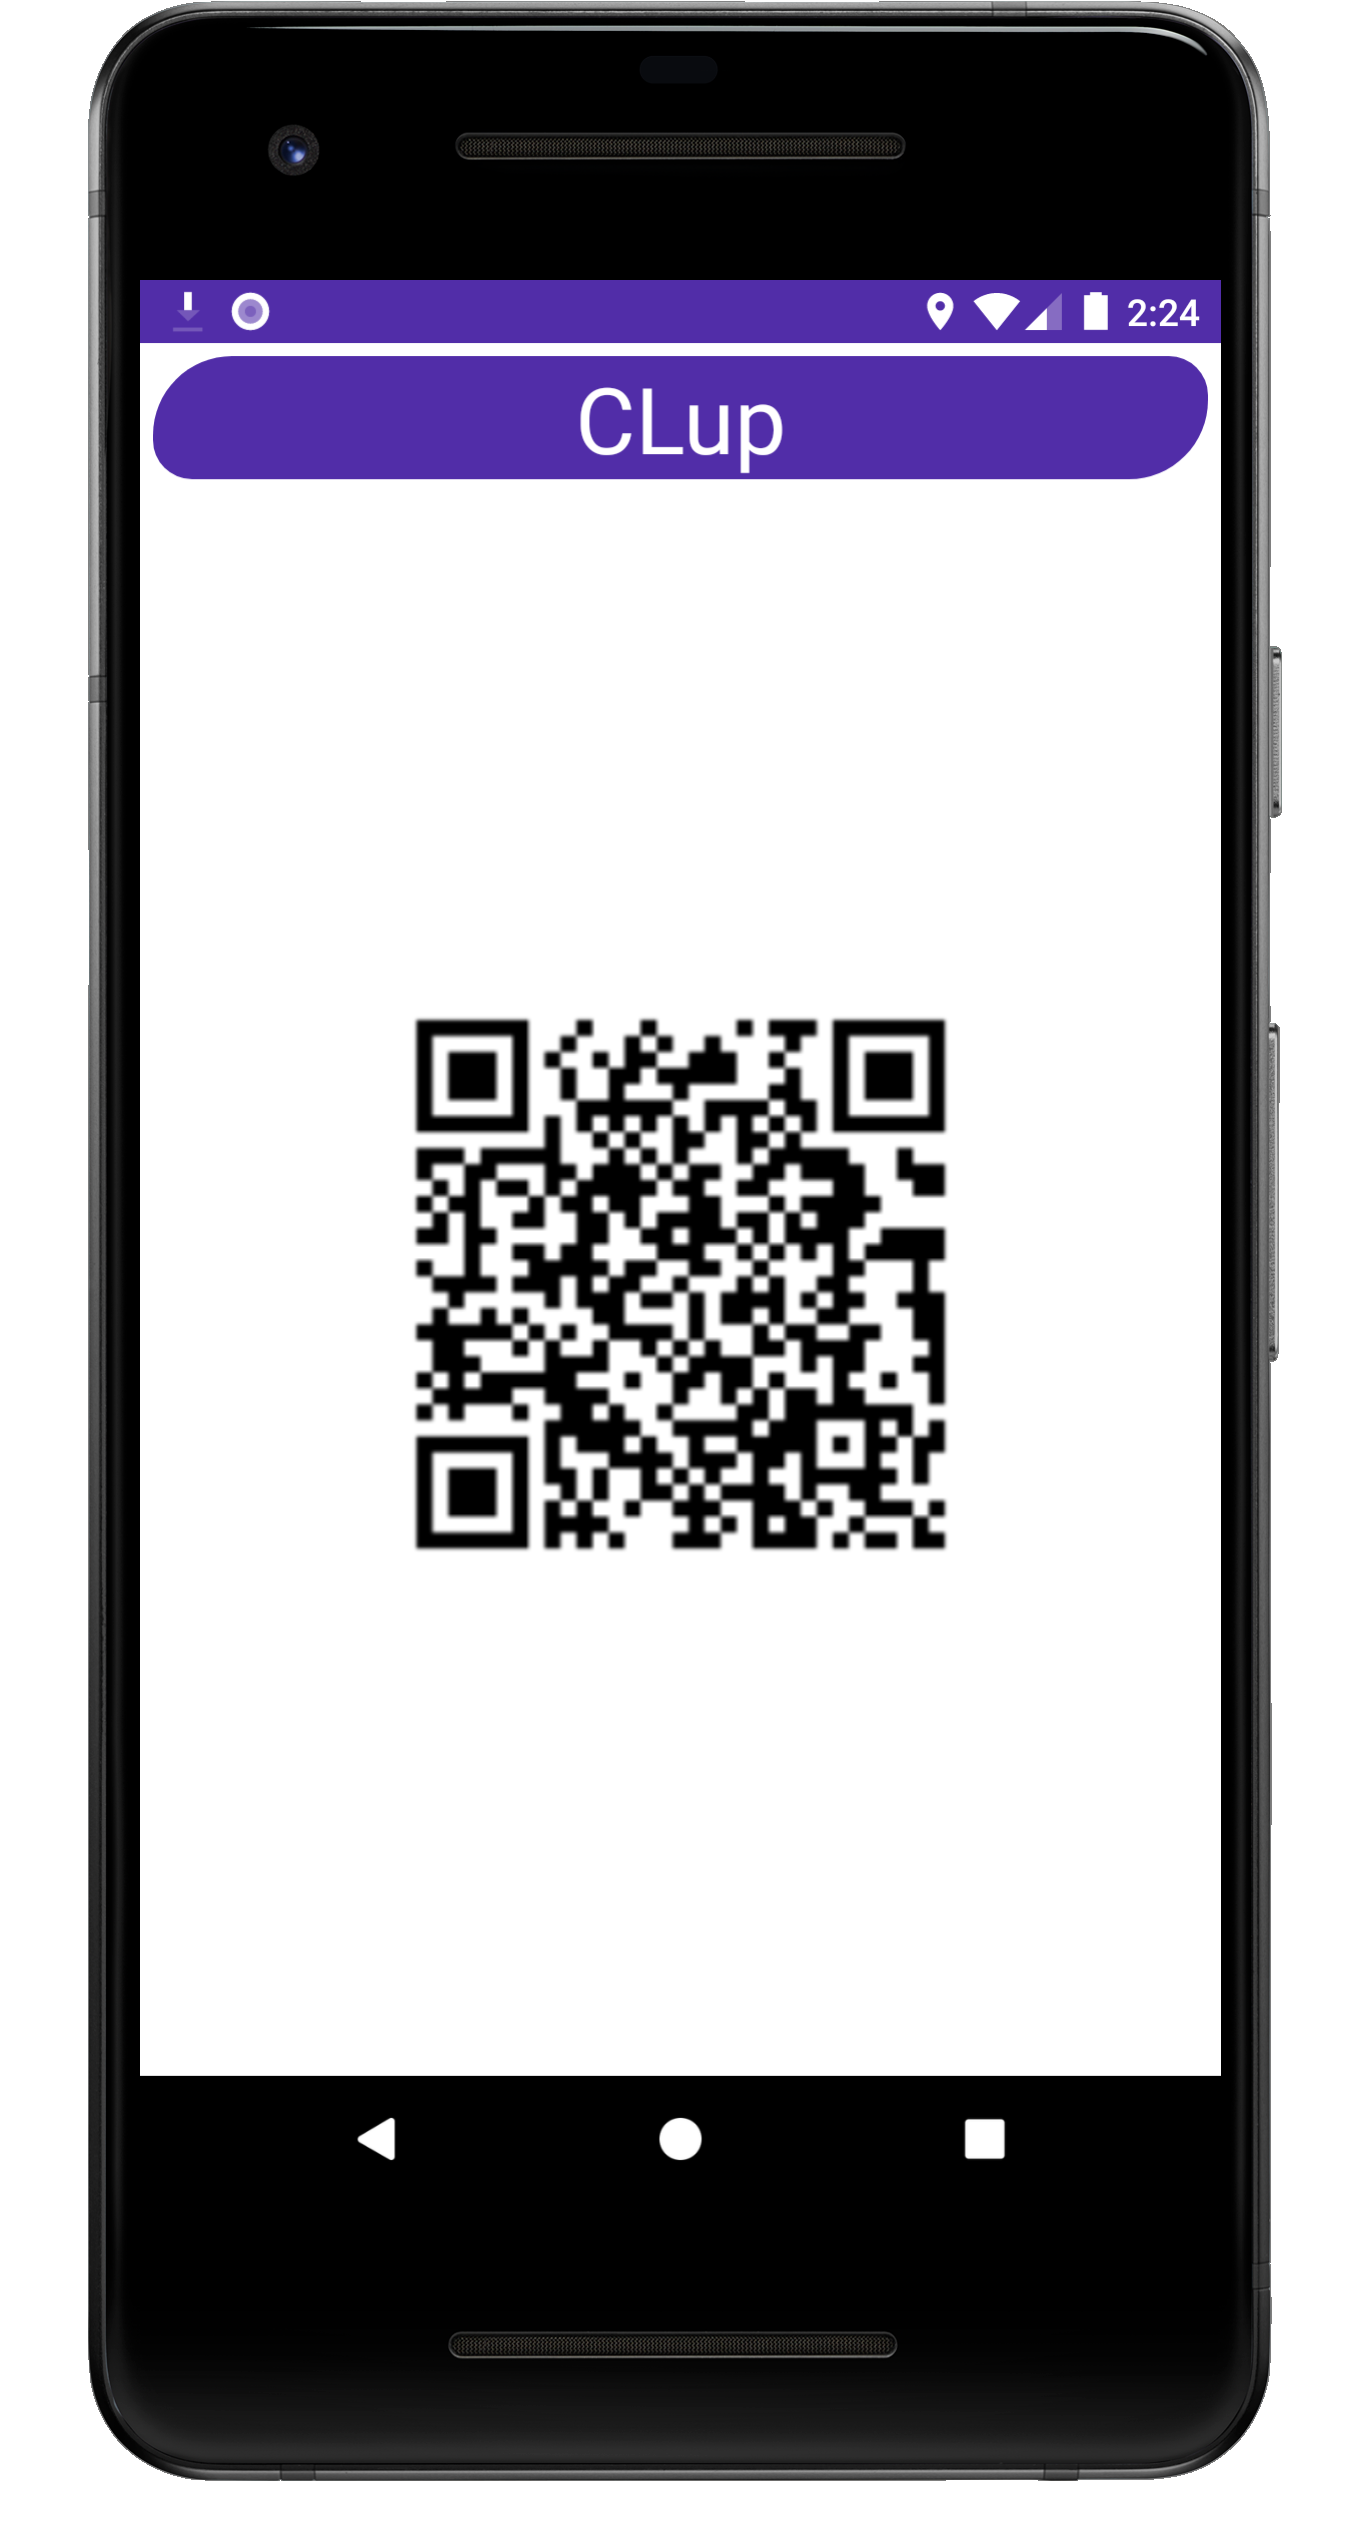
\includegraphics[width=0.4\textwidth]{images/show_qr_code.png}}
	\caption{Example of Get Status and Show QR code pages.}
\end{figure}

% TODO: add mokup for store manager

\subsection{Hardware Interfaces}

The system is distributed over three main hardware resources.

\begin{itemize}
	\item \textbf{Smartphone}: used by the customers that wants to line up or book a visit from remote. The smartphone has to have a \gls{gps} module to send the position and an Internet connection active to receive live updates by the server.
	\item \textbf{Physical spot}: is a totem composed by a tablet and a printer. The printer is a peripheral of the tablet. The tablet must have an Internet connection active.
	\item \textbf{Turnstile}: is used to control the entries. The tablet of the store manager, the QR code scanner and the display, that shows the next ticket numbers, are parts of the turnstile. More precisely, turnstile, scanner and display are peripherals of the tablet.
	We can imagine the turnstile as the metal detector in the airports, in which the guards are seated on the opposite side of the entrance.
	The store manager controls everything by the tablet and the tablet controls the peripherals under the constraints imposed by the store manager and the remote server.
	Indeed the tablet has to have an Internet connection active.
\end{itemize}

\subsection{Software interfaces}

The system, to work properly, needs external \gls{api}.

\begin{itemize}
	\item \textbf{Store \glspl{api}}: are well-liked if they there are. Additional data provided by the store, such as the history of the purchases of the customers, can be used to improve the quality of the estimations of the residence time; the sections of the store that will be visited by customers and so on.
	\item \textbf{Maps \glspl{api}}: can be used to improve the estimation of the needed time to arrive to the store by the global position of the customer.
\end{itemize}

\subsection{Communications Interfaces}

In this service we aren't not scheduling to use external communications interfaces.
Only the standard Internet protocols.

\section{Functional Requirements}

\subsection{Requirements}

Bla bla bla...

\begin{table}[H]
\centering
\begin{tabular}{| m{0.2\textwidth} | m{0.8\textwidth} |} 
	\hline
	\textbf{Goal} &
		\textbf{G1: Keep customers in safe condition w.r.t the \gls{dpcm} in force inside the store.} \\
	\hline
	\textbf{Requirements} &
		\begin{itemize}
			\item {\textbf{[R1]}}: The system has to schedule entrances to the store.
			\item {\textbf{[R2]}}: The system has to compute the maximum capacity of the store w.r.t. the social distances imposed by the \gls{dpcm} in force.
			\item {\textbf{[R3]}}: The system has to monitor the customers residence time in the store.
			\item {\textbf{[R4]}}: The system has to allow authorized customers to enter in the store.
			\item {\textbf{[R5]}}: The system has to deny unauthorized customers to enter in the store.
			\item {\textbf{[R6]}}: The system has to know when a customer enters in the store.
			\item {\textbf{[R7]}}: The system has to know when a customer has left the store.
		\end{itemize} \\
	\hline
	\shortstack[l]{\textbf{Domain} \\ \textbf{Assumptions}} & 
		\begin{itemize}
			\item {\textbf{[D1]}}: There is a \gls{dpcm} in force.
			\item {\textbf{[D2]}}: Customers follow the rules imposed by the \gls{dpcm} in force.
			\item {\textbf{[D3]}}: Customers enter in the store only if the system authorizes them.
			\item {\textbf{[D4]}}: Customers don't stay in the shop longer than necessary and they go away from the store after they have done their shopping.
			% \item {\textbf{[D]}}: If customers booked a visit to the store and they specify the category of grocery, they won't buy other things.
		\end{itemize} \\ 
	\hline
\end{tabular}
\end{table}

\begin{table}[H]
\centering
\begin{tabular}{| m{0.2\textwidth} | m{0.8\textwidth} |} 
	\hline
	\textbf{Goal} &
		\textbf{G2: Limit the physical line situation in the proximity of the store} \\
	\hline
	\textbf{Requirements} &
		\begin{itemize}
			\item {\textbf{[R8]}}: The system has to estimate the residence time, of a customer, in the store.
			\item {\textbf{[R9]}}: The system has to infer the residence time of the customers based on past purchases.
			\item {\textbf{[R10]}}: The system has to estimate the time needed to arrive, to the store, from the position of the customer.
			\item {\textbf{[R11]}}: The system has to track the global position of the customers.
			\item {\textbf{[R12]}}: The system has to release QR codes to the customers.
			\item {\textbf{[R13]}}: The system has to limit the number of releasable QR codes if imposed by the store manager.
			\item {\textbf{[R14]}}: The system has to allow the store manager to monitor the status of the queue.
			\item {\textbf{[R15]}}: The system has to notify customers about the remaining time to be authorized to enter in the store.
			\item {\textbf{[R16]}}: The system has to communicate which is the next served QR code number.
		\end{itemize} \\ 
	\hline
	\shortstack[l]{\textbf{Domain} \\ \textbf{Assumptions}} & 
		\begin{itemize}
			\item {\textbf{[D5]}}: Customers line up physically only if they have a valid (non expired) QR code.
			\item {\textbf{[D4]}}: Customers don't stay in the shop longer than necessary and they go away from the store after they have done their shopping.
			\item {\textbf{[D6]}}: Outside the store, there is space to queue.
		\end{itemize} \\ 
	\hline
\end{tabular}
\end{table}

\begin{table}[H]
\centering
\begin{tabular}{| m{0.2\textwidth} | m{0.8\textwidth} |} 
	\hline
	\textbf{Goal} &
		\textbf{G3: Allow customers to line up from a remote device.} \\
		% requirements per l'app e il servizio di prenotazione (quality standard)
	\hline
	\textbf{Requirements} &
		\begin{itemize}
			\item {\textbf{[R]}}: The system has to allow customers to register to the application.
			\item {\textbf{[R]}}: The system has to allow customers to login to the application.
			\item {\textbf{[R]}}: The system has to allow customers to get a QR code from the application.
			\item {\textbf{[R]}}: The system has to release QR codes to the customers through the application.
			\item {\textbf{[R]}}: The system has to alert customers if the queue is full.
			\item {\textbf{[R]}}: The system has to encode the lining up number in the QR code.
			\item {\textbf{[R]}}: The system has to allow customers to watch the QR code from the application.
			\item {\textbf{[R]}}: The system has to allow customers to watch the lining up number encoded in the QR code.
			\item {\textbf{[R]}}: The system has to allow customers to watch the remaining time to be authorized to enter in the store.
			\item {\textbf{[R]}}: The system has to update the remaining time showed to the customers.
			\item {\textbf{[R]}}: The system has to allow customers to delete a lining up operation.
			\item {\textbf{[R]}}: The system has to notify customers about the validation status of the QR code.
			\item {\textbf{[R]}}: The system has to check if customers have Internet connection active.
			\item {\textbf{[R]}}: The system has to check if customers have allowed the permissions requested by the application.
		\end{itemize} \\ 
	\hline
	\shortstack[l]{\textbf{Domain} \\ \textbf{Assumptions}} & 
		\begin{itemize}
			\item {\textbf{[D]}}: Customers have a smartphone.
			\item {\textbf{[D]}}: Customers have installed the \gls{clup} application.
			\item {\textbf{[D]}}: Customers allow the permissions requested by the application.
			\item {\textbf{[D]}}: Customers keep Internet connection active.
		\end{itemize} \\ 
	\hline
\end{tabular}
\end{table}

\begin{table}[H]
\centering
\begin{tabular}{| m{0.2\textwidth} | m{0.8\textwidth} |} 
	\hline
	\textbf{Goal} &
		\textbf{G4: Allow store manager to monitor entrances.} \\
	\hline
	\textbf{Requirements} &
		\begin{itemize}
			\item {\textbf{[R]}}: The system has to register store managers in the application.
			\item {\textbf{[R]}}: The system has to allow store managers to login to the application.
			\item {\textbf{[R]}}: The system has to allow store managers to monitor the status of the queue.
			\item {\textbf{[R]}}: The system has to allow store managers to limit the number of QR codes released.
			\item {\textbf{[R]}}: The system has to allow store managers to monitor the number of customers inside the store.
			\item {\textbf{[R]}}: The system has to scan the QR codes of the customers.
			\item {\textbf{[R]}}: The system has to allow store managers to modify the timing parameters of the scheduler.
			\item {\textbf{[R]}}: The system has to check if store managers have Internet connection active.
			\item {\textbf{[R]}}: The system has to check if store managers have allowed the permissions requested by the application.
		\end{itemize} \\ 
	\hline
	\shortstack[l]{\textbf{Domain} \\ \textbf{Assumptions}} & 
		\begin{itemize}
			\item {\textbf{[D]}}: There is a store manager present in the store.
			\item {\textbf{[D]}}: Store managers allow the permissions requested by the application.
			\item {\textbf{[D]}}: Store managers keep Internet connection active.
		\end{itemize} \\ 
	\hline
\end{tabular}
\end{table}

\begin{table}[H]
\centering
\begin{tabular}{| m{0.2\textwidth} | m{0.8\textwidth} |} 
	\hline
	\textbf{Goal} &
		\textbf{G5: Allow customers to line up from a physical spot.} \\
	\hline
	\textbf{Requirements} &
		\begin{itemize}
			\item {\textbf{[R]}}: The system has to allow unregistered customers to line up.
			\item {\textbf{[R]}}: The system has to allow customers to get a QR code from a physical spot.
			\item {\textbf{[R]}}: The system has to release QR codes to the customers through the physical spot.
			\item {\textbf{[R]}}: The system has to encode the lining up number in the QR code.
			\item {\textbf{[R]}}: The system has to print QR codes on a paper tickets.
			\item {\textbf{[R]}}: The system has to alert customers if the queue is full.
			\item {\textbf{[R]}}: The system has to alert when the paper and toner of the physical spot is going to finish.
		\end{itemize} \\ 
	\hline
	\shortstack[l]{\textbf{Domain} \\ \textbf{Assumptions}} & 
		\begin{itemize}
			\item {\textbf{[D]}}: Physical spots are powered on every working day.
			\item {\textbf{[D]}}: Physical spots are refilled when asked by the system. 
		\end{itemize} \\ 
	\hline
\end{tabular}
\end{table}

\begin{table}[H]
\centering
\begin{tabular}{| m{0.2\textwidth} | m{0.8\textwidth} |} 
	\hline
	\textbf{Goal} &
		\textbf{G6: Allow customers to book a visit from a remote device.} \\
		% requirements che implicano l'implementazione di una schermata nell'app per la prenotazione
	\hline
	\textbf{Requirements} &
		\begin{itemize}
			\item {\textbf{[R]}}: The system has to allow customers to register to the application.
			\item {\textbf{[R]}}: The system has to allow customers to login to the application.
			\item {\textbf{[R]}}: The system has to allow customers to get a QR code from the application.
			\item {\textbf{[R]}}: The system has to allow customers to specify the date and time for a visit to the store.
			\item {\textbf{[R]}}: The system has to allow customers to specify the category of grocery they want to buy.
			\item {\textbf{[R]}}: The system has to release QR codes to the customers through the application.
			\item {\textbf{[R]}}: The system has to alert customers if the queue is full.
			\item {\textbf{[R]}}: The system has to encode the book-a-visit number in the QR code.
			\item {\textbf{[R]}}: The system has to allow customers to watch the QR code from the application.
			\item {\textbf{[R]}}: The system has to allow customers to watch the book-a-visit number encoded in the QR code.
			\item {\textbf{[R]}}: The system has to allow customers to watch the remaining time to be authorized to enter in the store.
			\item {\textbf{[R]}}: The system has to allow customers to delete a book-a-visit operation.
			\item {\textbf{[R]}}: The system has to notify customers about the validation status of the QR code.
			\item {\textbf{[R]}}: The system has to check if customers have Internet connection active.
			\item {\textbf{[R]}}: The system has to check if customers have allowed the permissions requested by the application.
		\end{itemize} \\ 
	\hline
	\shortstack[l]{\textbf{Domain} \\ \textbf{Assumptions}} & 
		\begin{itemize}
			\item {\textbf{[D]}}: Customers have a smartphone.
			\item {\textbf{[D]}}: Customers have installed the \gls{clup} application.
			\item {\textbf{[D]}}: Customers allow the permissions requested by the application.
			\item {\textbf{[D]}}: Customers keep Internet connection active.
		\end{itemize} \\ 
	\hline
\end{tabular}
\end{table}


\subsection{Definition of Use Case Diagrams}

Bla bla bla...

\begin{figure}[H]
	\centering
	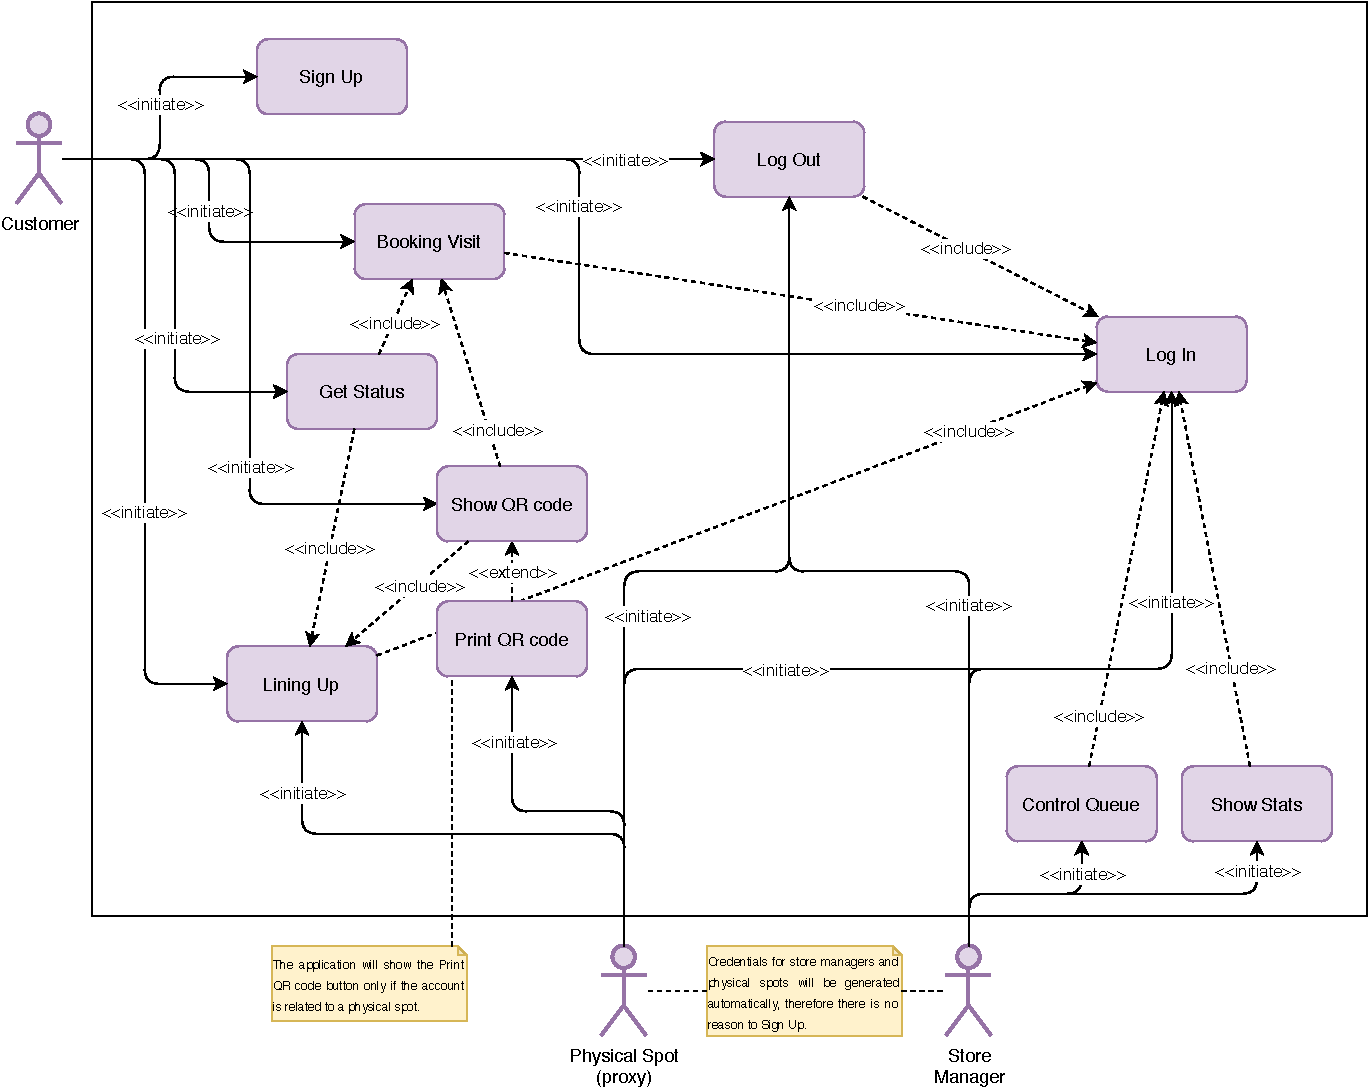
\includegraphics[width=1.0\textwidth]{images/use_cases_diagram.pdf}
	\caption{Use cases diagram.}
\end{figure}

\begin{table}[H]
\centering
\begin{tabular}{| m{0.3\textwidth} | m{0.7\textwidth} |} 
	\hline
	\textbf{Name} & Sign Up \\ 
	\hline
	\textbf{Actor} & Customer \\ 
	\hline
	\textbf{Entry Conditions} & Customer is on the Sign Up page. \\ 
	\hline
	\textbf{Event Flows} &
	\begin{itemize}
		\item Customer inserts the requested information in the form.
		\item Customer clicks on the Sign Up button.
	\end{itemize} \\ 
	\hline
	\textbf{Exit Conditions} & Sign Up completed successfully and customer is logged in, then the application shows the Home page. \\ 
	\hline
	\textbf{Exceptions} &
	\begin{itemize}
		\item Customer's username already in use.
		\item Empty form field.
		\item Policy agreement rejected.
		\item Lost Internet connection.
	\end{itemize} \\ 
	\hline
\end{tabular}
\caption{Use case: \textbf{Sign Up}.}
\label{tableSignUp}
\end{table}

\begin{table}[H]
\centering
\begin{tabular}{| m{0.3\textwidth} | m{0.7\textwidth} |} 
	\hline
	\textbf{Name} & Log In \\ 
	\hline
	\textbf{Actor} & Customer - Physical Spot - Store Manager \\ 
	\hline
	\textbf{Entry Conditions} & Actor is on the Log In page. \\ 
	\hline
	\textbf{Event Flows} &
	\begin{itemize}
	\item Actor inserts the requested information in the form.
	\item Actor clicks on the Log In button.
	\end{itemize} \\ 
	\hline
	\textbf{Exit Conditions} & Log In completed successfully and actor is redirected to the Home page. \\ 
	\hline
	\textbf{Exceptions} &
	\begin{itemize}
	\item Actor's username or password incorrect.
	\item Empty form field.
	\item Lost Internet connection.
	\end{itemize} \\ 
	\hline
\end{tabular}
\caption{Use case: \textbf{Log In}.}
\label{tableLogIn}
\end{table}

\begin{table}[H]
\centering
\begin{tabular}{| m{0.3\textwidth} | m{0.7\textwidth} |} 
	\hline
	\textbf{Name} & Log Out \\ 
	\hline
	\textbf{Actor} & Customer - Physical Spot - Store Manager \\ 
	\hline
	\textbf{Entry Conditions} & Actor is on the Log Out page. \\ 
	\hline
	\textbf{Event Flows} &
	\begin{itemize}
	\item Actor clicks on the Log Out button.
	\end{itemize} \\ 
	\hline
	\textbf{Exit Conditions} & Log Out completed successfully and actor is redirected to the Log In page. \\ 
	\hline
	\textbf{Exceptions} &
	\begin{itemize}
	\item Actor already logged out.
	\item Lost Internet connection.
	\end{itemize} \\ 
	\hline
\end{tabular}
\caption{Use case: \textbf{Log Out}.}
\label{tableLogOut}
\end{table}

\begin{table}[H]
\centering
\begin{tabular}{| m{0.3\textwidth} | m{0.7\textwidth} |} 
	\hline
	\textbf{Name} & Lining Up \\ 
	\hline
	\textbf{Actor} & Customer - Physical Spot \\ 
	\hline
	\textbf{Entry Conditions} & Actor is on the Home page. \\ 
	\hline
	\textbf{Event Flows} &
	\begin{itemize}
	\item Actor clicks on the Lining Up button.
	\item Actor inserts the requested data in the form.
	\item Actor clicks on the confirmation button.
	\end{itemize} \\ 
	\hline
	\textbf{Exit Conditions} & Lining Up completed successfully, the application returns the Status page. \\ 
	\hline
	\textbf{Exceptions} &
	\begin{itemize}
	\item Previous Lining Up action was not expired (only in case of remote customer).
	\item Previous Booking Visit action was not expired (only in case of remote customer).
	\item Actor wasn't logged.
	\item Lost Internet connection.
	\end{itemize} \\ 
	\hline
\end{tabular}
\caption{Use case: \textbf{Lining Up}.}
\label{tableLiningUp}
\end{table}

\begin{table}[H]
\centering
\begin{tabular}{| m{0.3\textwidth} | m{0.7\textwidth} |} 
	\hline
	\textbf{Name} & Booking Visit \\ 
	\hline
	\textbf{Actor} & Customer \\ 
	\hline
	\textbf{Entry Conditions} & Customer is on the Home page. \\ 
	\hline
	\textbf{Event Flows} &
	\begin{itemize}
	\item Customer clicks on the Booking Visit button.
	\item Customer fills the form with the requested data.
	\item Customer clicks on the Submit button.
	\end{itemize} \\ 
	\hline
	\textbf{Exit Conditions} & Booking Visit completed successfully and the application returns, to the customer, the Status page. \\ 
	\hline
	\textbf{Exceptions} &
	\begin{itemize}
	\item Previous Lining Up action was not expired.
	\item Previous Booking Visit action was not expired.
	\item Customer wasn't logged.
	\item Lost Internet connection.
	\end{itemize} \\ 
	\hline
\end{tabular}
\caption{Customer - use case: \textbf{Booking Visit}.}
\label{tableBookingVisit}
\end{table}

\begin{table}[H]
\centering
\begin{tabular}{| m{0.3\textwidth} | m{0.7\textwidth} |} 
	\hline
	\textbf{Name} & Show QR code - Print QR code \\ 
	\hline
	\textbf{Actor} & Customer - Physical Spot \\ 
	\hline
	\textbf{Entry Conditions} & Actor is on the Home page. \\ 
	\hline
	\textbf{Event Flows} &
	\begin{itemize}
	\item Actor clicks on the Show QR (Print QR) code button.
	\end{itemize} \\ 
	\hline
	\textbf{Exit Conditions} & The application shows (print) the QR code. \\ 
	\hline
	\textbf{Exceptions} &
	\begin{itemize}
	\item QR code wasn't saved on the application correctly (only in case of remote customer).
	\item No Lining Up, or Booking Visit, action previously performed (only in case of remote customer).
	\item Actor wasn't logged.
	\item Spot finished the paper.
	\item Spot finished the ink.
	\end{itemize} \\ 
	\hline
\end{tabular}
\caption{Use case: \textbf{Show QR code - Print QR code}.}
\label{tableShowQR}
\end{table}

\begin{table}[H]
\centering
\begin{tabular}{| m{0.3\textwidth} | m{0.7\textwidth} |} 
	\hline
	\textbf{Name} & Get Status \\ 
	\hline
	\textbf{Actor} & Customer \\ 
	\hline
	\textbf{Entry Conditions} & Customer is on the Home page. \\ 
	\hline
	\textbf{Event Flows} &
	\begin{itemize}
	\item Customer clicks on the Get Status button.
	\end{itemize} \\ 
	\hline
	\textbf{Exit Conditions} & The application returns the Get Status page showing information about the last Lining Up, or Booking Visit, operation. \\ 
	\hline
	\textbf{Exceptions} &
	\begin{itemize}
	\item No operation previously performed, therefore there is no data to show.
	\item Customer wasn't logged.
	\item Lost Internet connection.
	\end{itemize} \\ 
	\hline
\end{tabular}
\caption{Customer - use case: \textbf{Get Status}.}
\label{tableGetStatus}
\end{table}

\begin{table}[H]
\centering
\begin{tabular}{| m{0.3\textwidth} | m{0.7\textwidth} |} 
	\hline
	\textbf{Name} & Control Queue \\ 
	\hline
	\textbf{Actor} & Store Manager \\ 
	\hline
	\textbf{Entry Conditions} & Store Manager is on the Home page. \\ 
	\hline
	\textbf{Event Flows} &
	\begin{itemize}
	\item Store Manager clicks on the Control Queue button.
	\end{itemize} \\ 
	\hline
	\textbf{Exit Conditions} & The application returns the Control Queue page showing options to manage the queue. \\ 
	\hline
	\textbf{Exceptions} &
	\begin{itemize}
	\item Store Manager wasn't logged.
	\item Lost Internet connection.
	\end{itemize} \\ 
	\hline
\end{tabular}
\caption{Store Manager - use case: \textbf{Control Queue}.}
\label{tableGetStatus}
\end{table}

\begin{table}[H]
\centering
\begin{tabular}{| m{0.3\textwidth} | m{0.7\textwidth} |} 
	\hline
	\textbf{Name} & Show Stats \\ 
	\hline
	\textbf{Actor} & Store Manager \\ 
	\hline
	\textbf{Entry Conditions} & Store Manager is on the Home page. \\ 
	\hline
	\textbf{Event Flows} &
	\begin{itemize}
	\item Store Manager clicks on the Show Stats button.
	\end{itemize} \\ 
	\hline
	\textbf{Exit Conditions} & The application returns the Show Stats page showing information about the number of customers inside the store, the length of the queue and other information about the waiting time in queue. \\ 
	\hline
	\textbf{Exceptions} &
	\begin{itemize}
	\item Store Manager wasn't logged.
	\item Lost Internet connection.
	\end{itemize} \\ 
	\hline
\end{tabular}
\caption{Store Manager - use case: \textbf{Show Stats}.}
\label{tableGetStatus}
\end{table}


\subsection{Use Cases and Sequence/Activity Diagrams}

\begin{figure}[H]
	\centering
	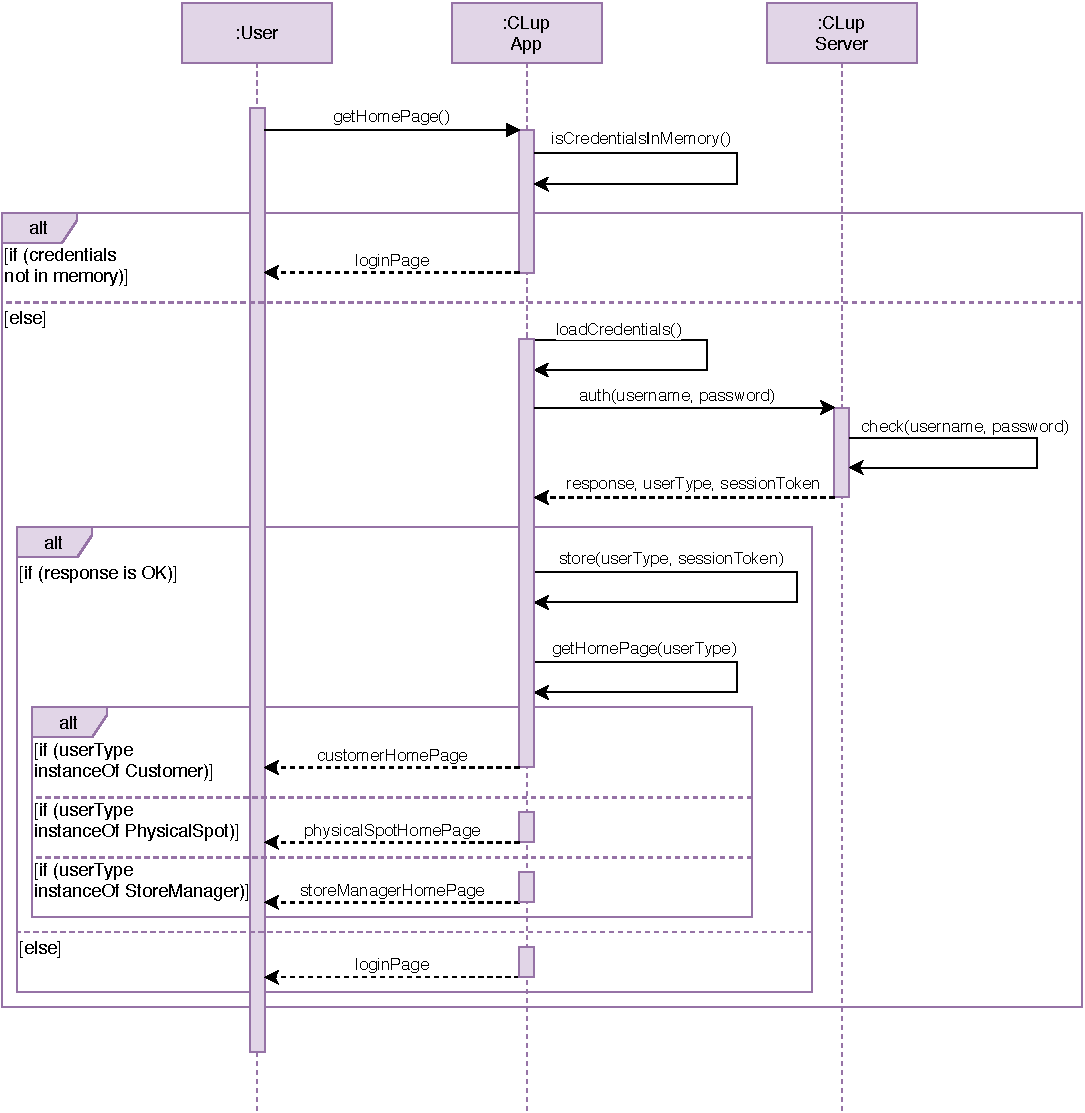
\includegraphics[width=1.0\textwidth]{images/getHomePage_sequence_diagram.pdf}
	\caption{Home page sequence diagram.}
\end{figure}

\begin{figure}[H]
	\centering
	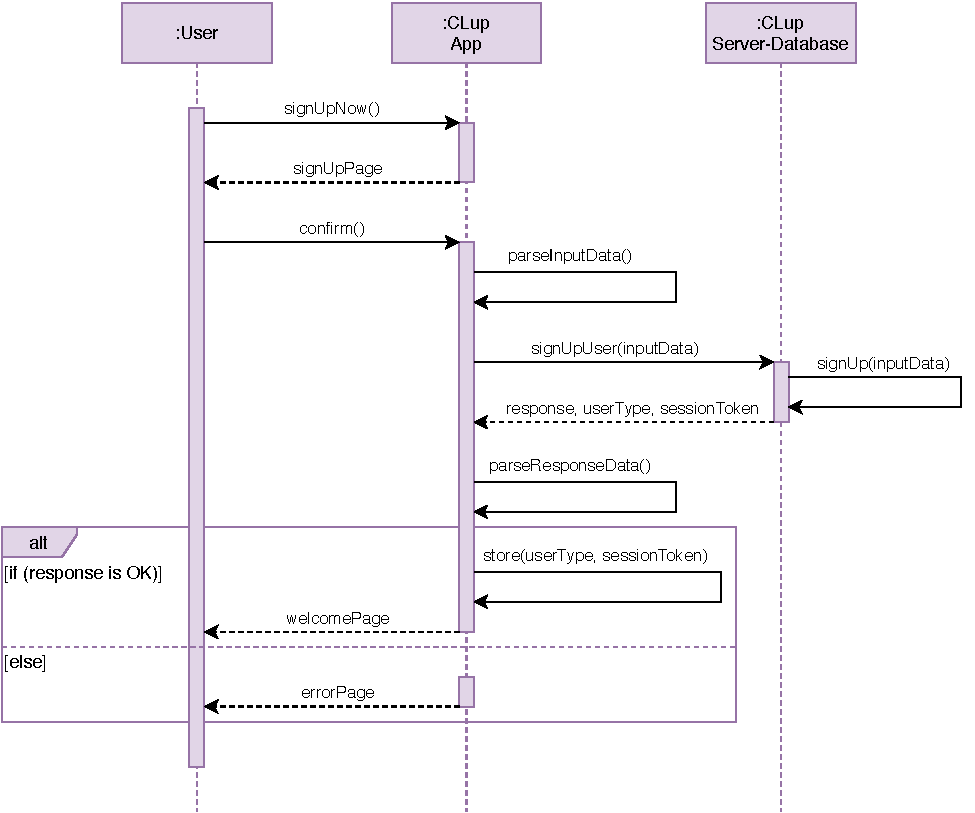
\includegraphics[width=1.0\textwidth]{images/signUp_sequence_diagram.pdf}
	\caption{Sign Up sequence diagram.}
\end{figure}

\begin{figure}[H]
	\centering
	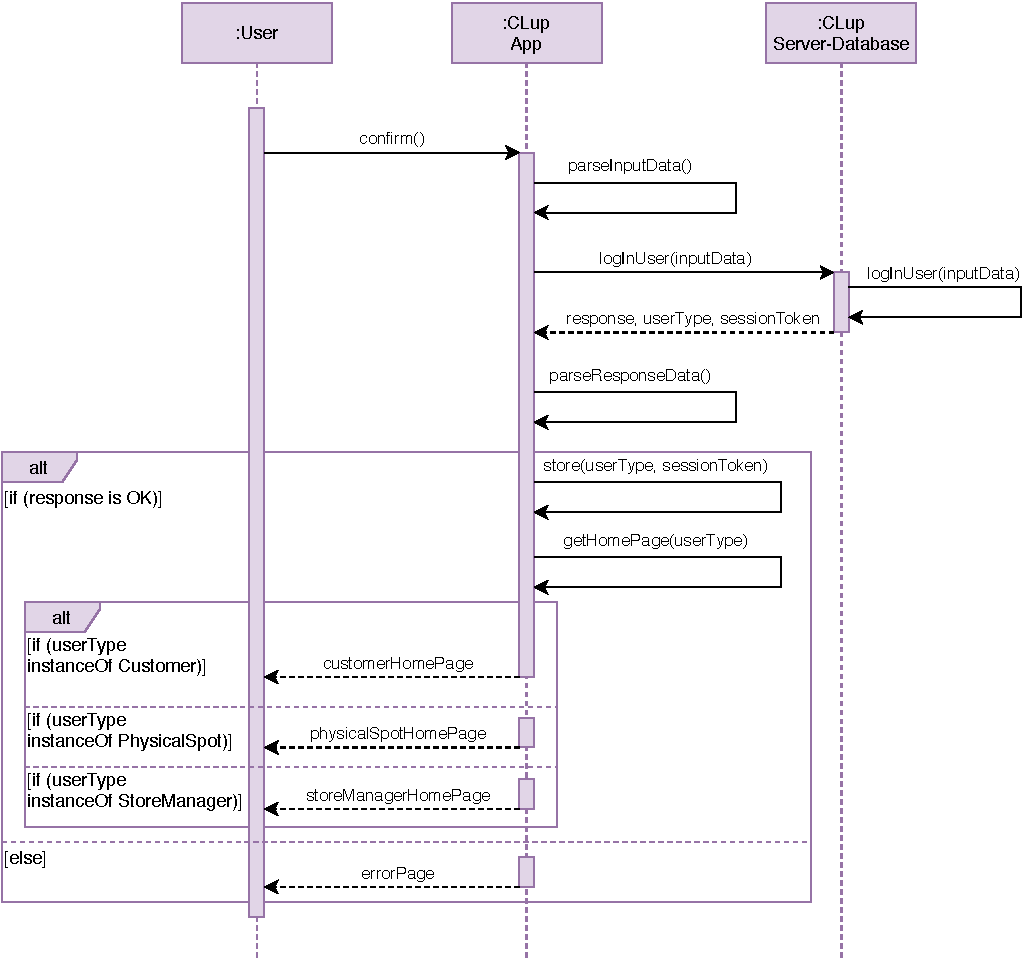
\includegraphics[width=1.0\textwidth]{images/logIn_sequence_diagram.pdf}
	\caption{Log In sequence diagram.}
\end{figure}

\begin{figure}[H]
	\centering
	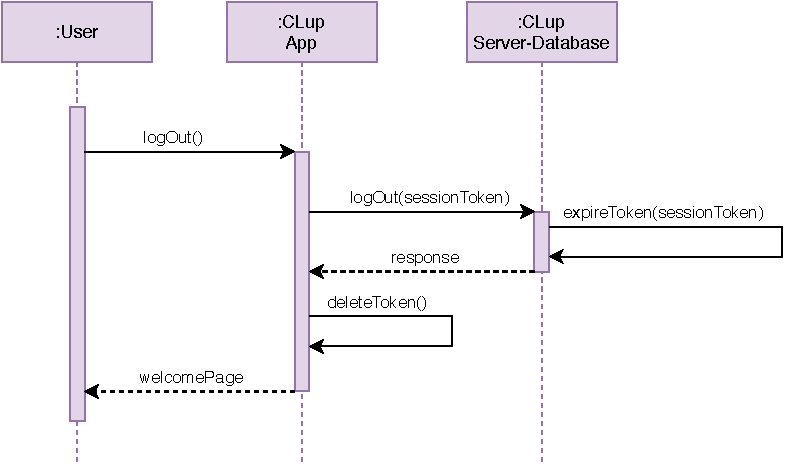
\includegraphics[width=1.0\textwidth]{images/logOut_sequence_diagram.pdf}
	\caption{Log Out sequence diagram.}
\end{figure}

\begin{figure}[H]
	\centering
	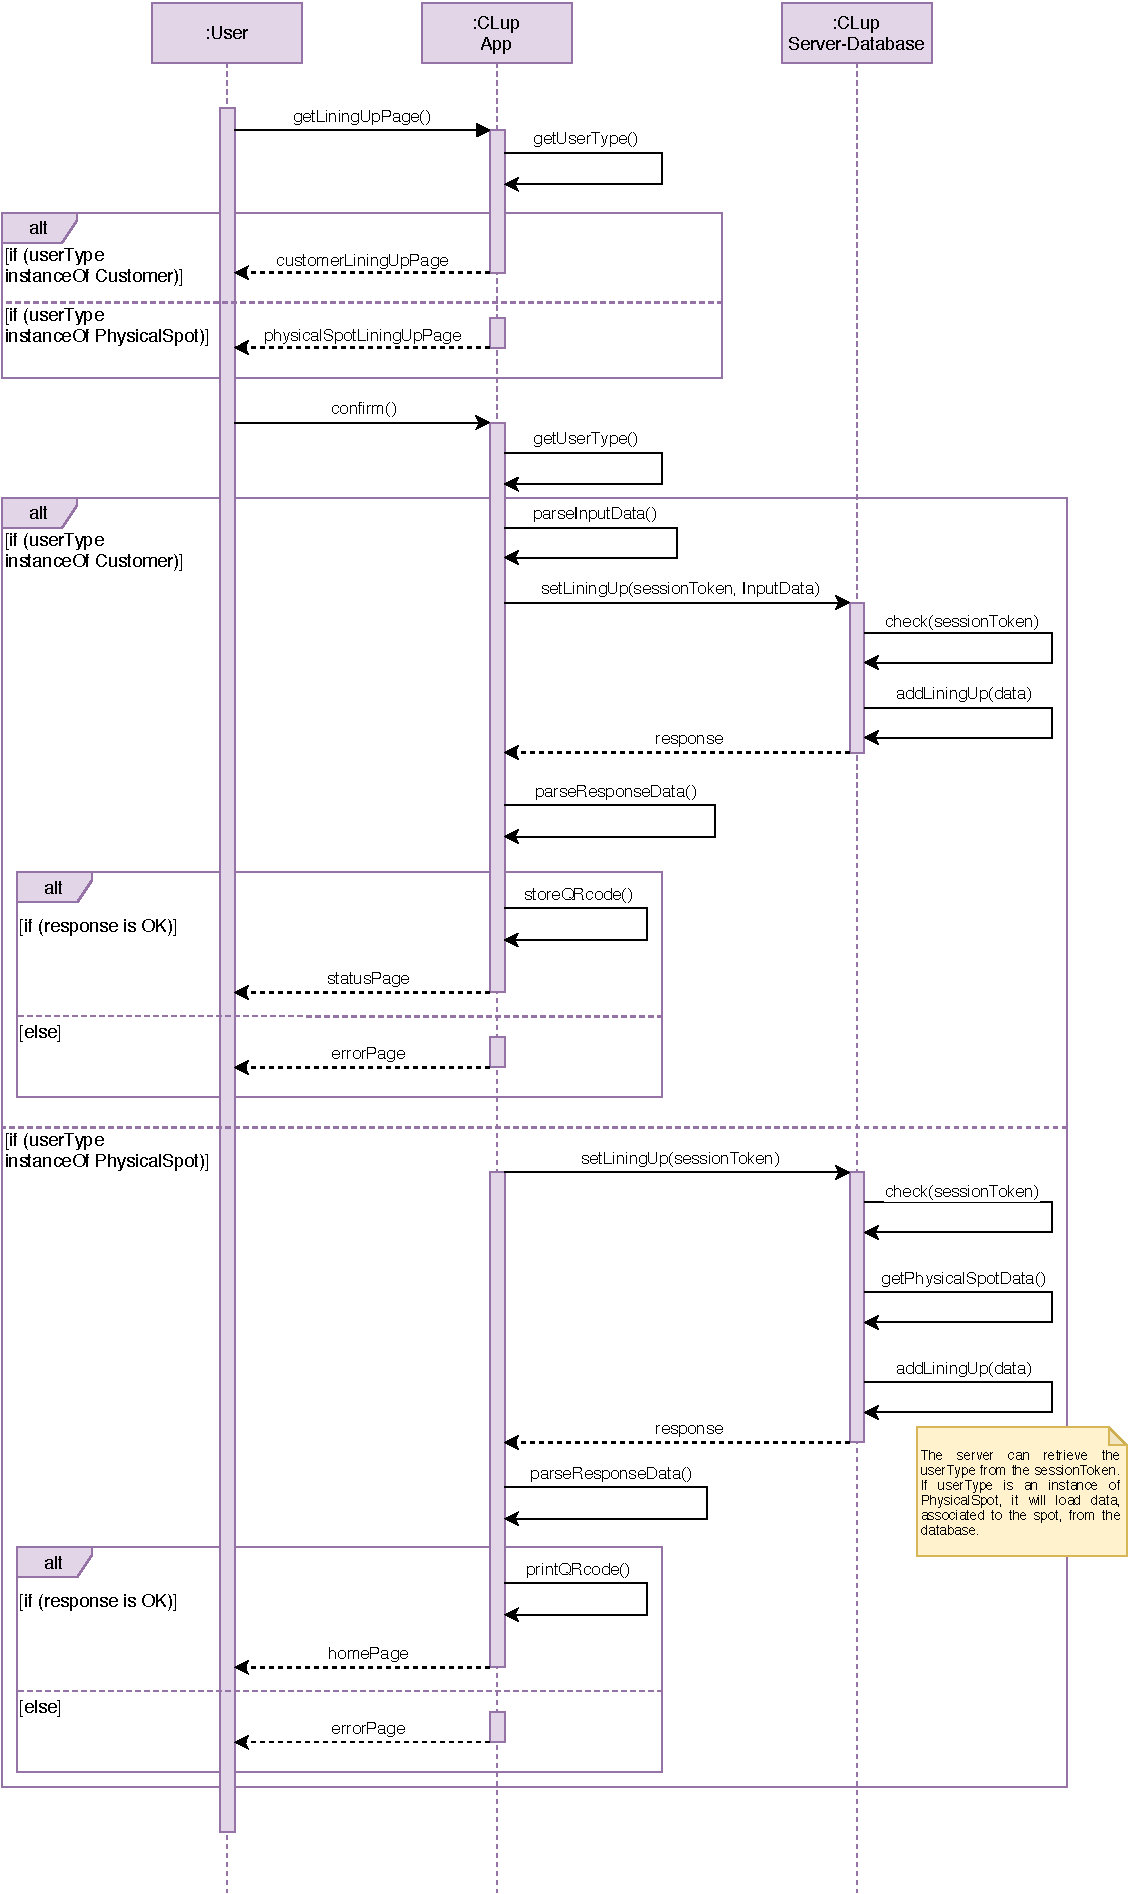
\includegraphics[width=1.0\textwidth]{images/liningUp_sequence_diagram.pdf}
	\caption{Lining Up sequence diagram.}
	\label{figure:liningUpSequenceDiagram}
\end{figure}

\begin{figure}[H]
	\centering
	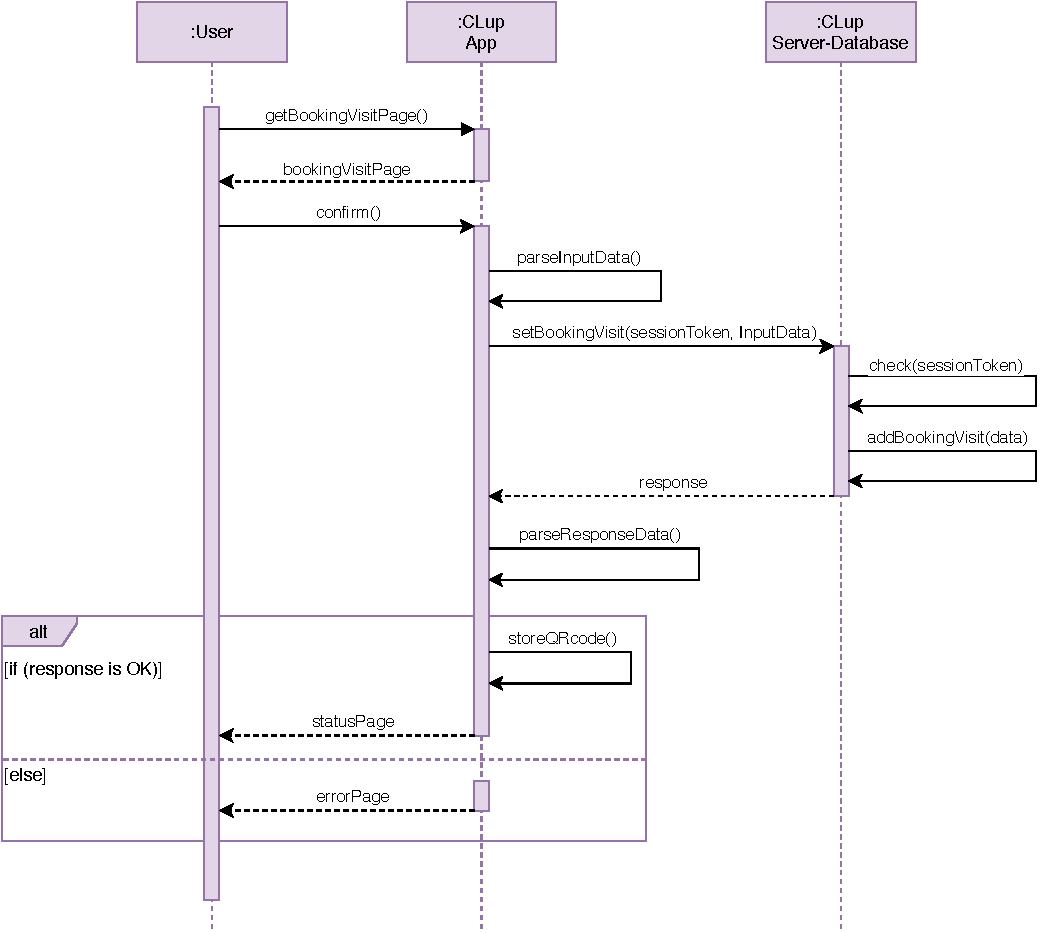
\includegraphics[width=1.0\textwidth]{images/bookingVisit_sequence_diagram.pdf}
	\caption{Booking a Visit sequence diagram.}
\end{figure}

\begin{figure}[H]
	\centering
	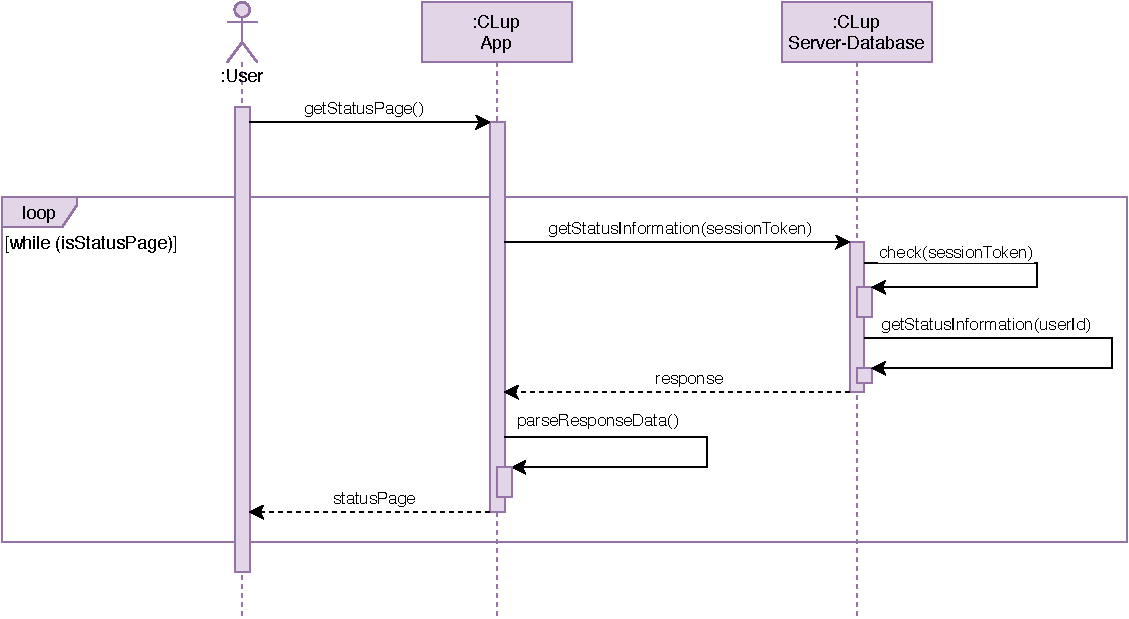
\includegraphics[width=1.0\textwidth]{images/getStatusPage_sequence_diagram.pdf}
	\caption{Get Status sequence diagram.}
\end{figure}

\begin{figure}[H]
	\centering
	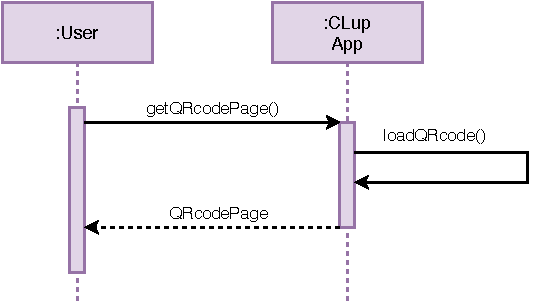
\includegraphics[width=1.0\textwidth]{images/getQRcodePage_sequence_diagram.pdf}
	\caption{QR code page sequence diagram.}
\end{figure}

\begin{figure}[H]
	\centering
	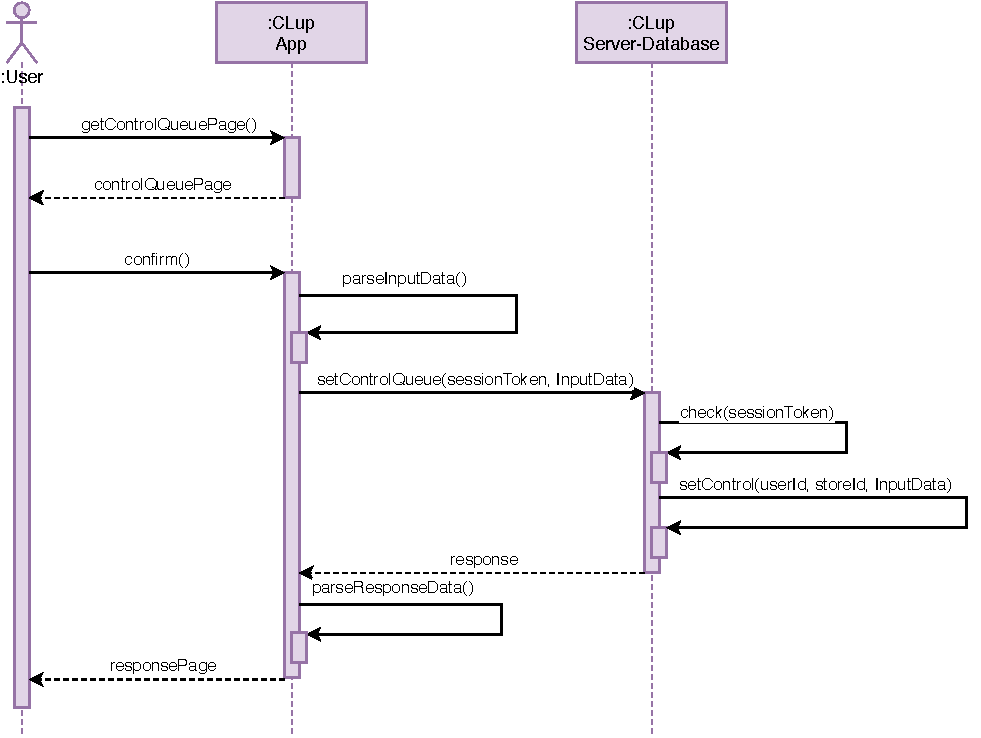
\includegraphics[width=1.0\textwidth]{images/getControlQueuePage_sequence_diagram.pdf}
	\caption{Control Queue sequence diagram.}
\end{figure}

\begin{figure}[H]
	\centering
	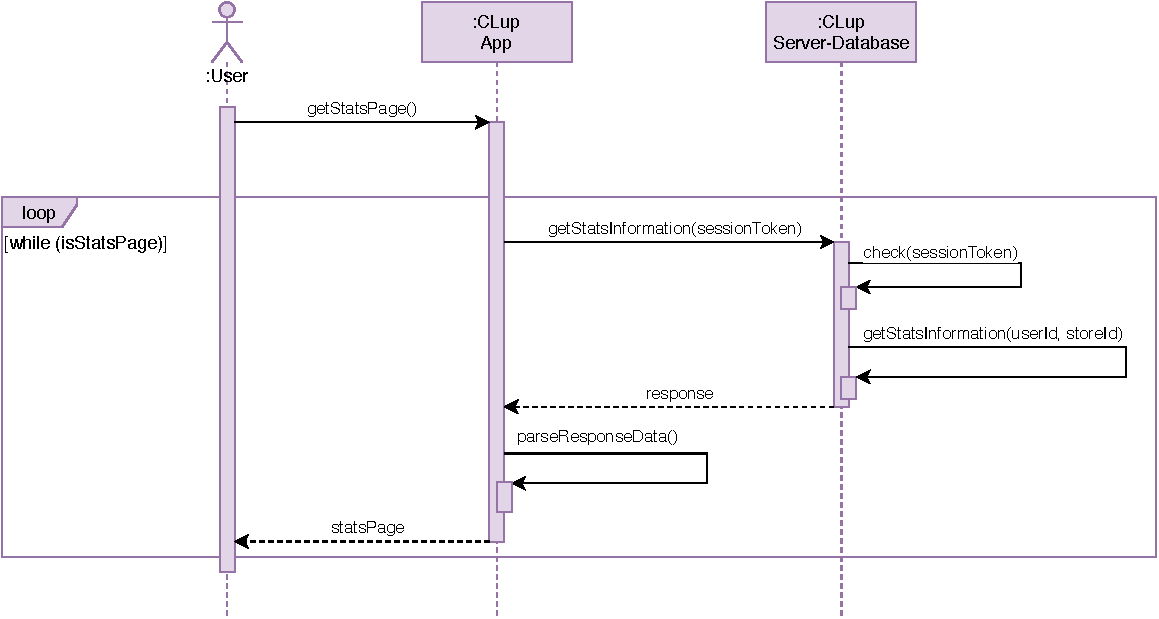
\includegraphics[width=1.0\textwidth]{images/getShowStatsPage_sequence_diagram.pdf}
	\caption{Show Stats sequence diagram.}
\end{figure}

\subsection{Mapping on Requirements}

\section{Performance Requirements}

\section{Design Constraints}

\subsection{Standard Compliance}
\subsection{Hardware limitations}
\subsection{Any Other Constraint}

\section{Software System Attributes}

\subsection{Reliability}
\subsection{Availability}
\subsection{Security}
\subsection{Maintainability}
\subsection{Portability}
\chapter{Formal Analysis Using Alloy}

\section{Alloy Code}

In this section is shown the alloy code that represent some parts of Clup model. The representation focus mainly on how the queue works with different kind of users, from the moment the line-up and so they appear inside this model to the moment they enter inside the store. Their place in the queue is represented by their ticket that encodes inside the QR code the information of lining-up and so of the user. That it is used to recognize the place that a person has in the queue and so to allow only the correct one to enter the store.
It is also shown by the Alloy’s graphic tool some worlds that evidence how the different components of the model and their properties work with each other in different context. And some properties are checked by using the assertion feature. 


\lstinputlisting[language=Alloy]{alloy/Clup_final.als}

\begin{figure}[H]
	\centering
	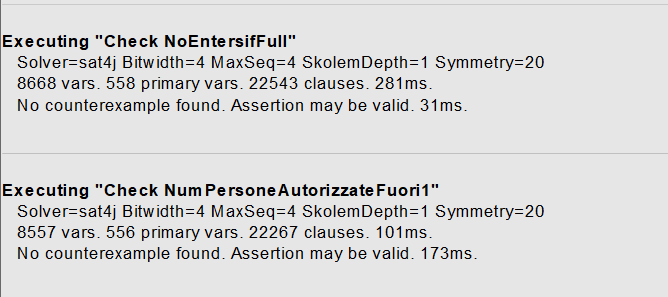
\includegraphics[width=\textwidth]{images/Assertions.png}
	\caption{Assertions verification}
	\label{figure: Assertions verification}
\end{figure}

\begin{sidewaysfigure}
	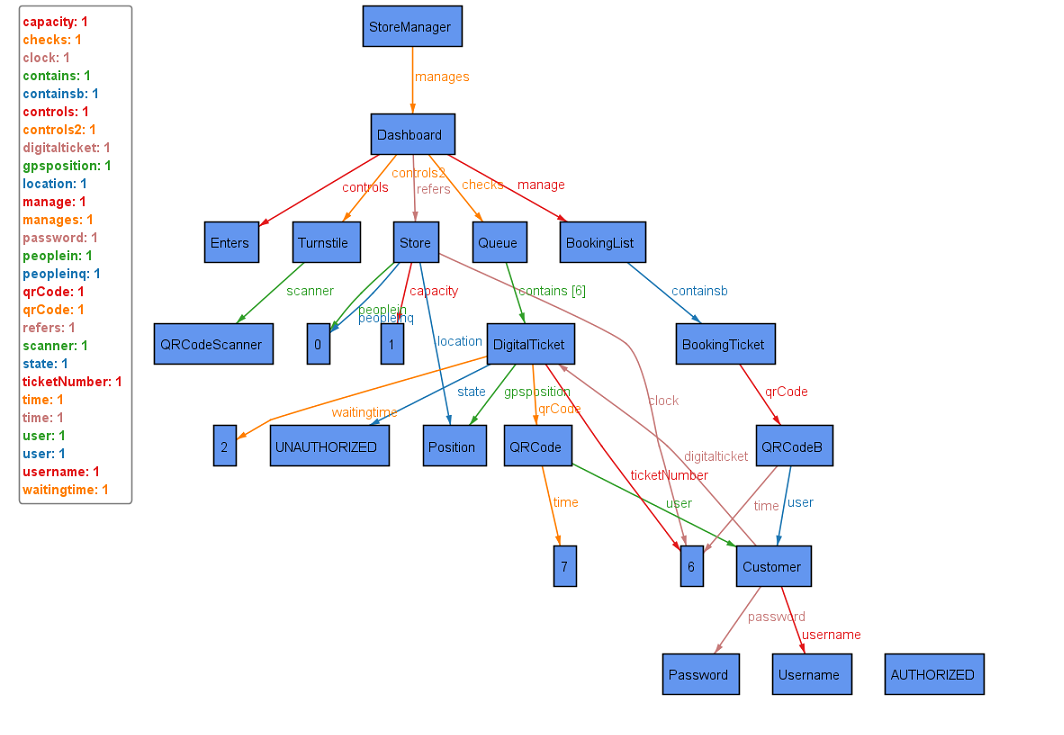
\includegraphics[width=1.0\textwidth]{images/AlloyW1.png}
	\caption{World1.}
	\label{figure: World1}
\end{sidewaysfigure}

\begin{sidewaysfigure}
	\centering
	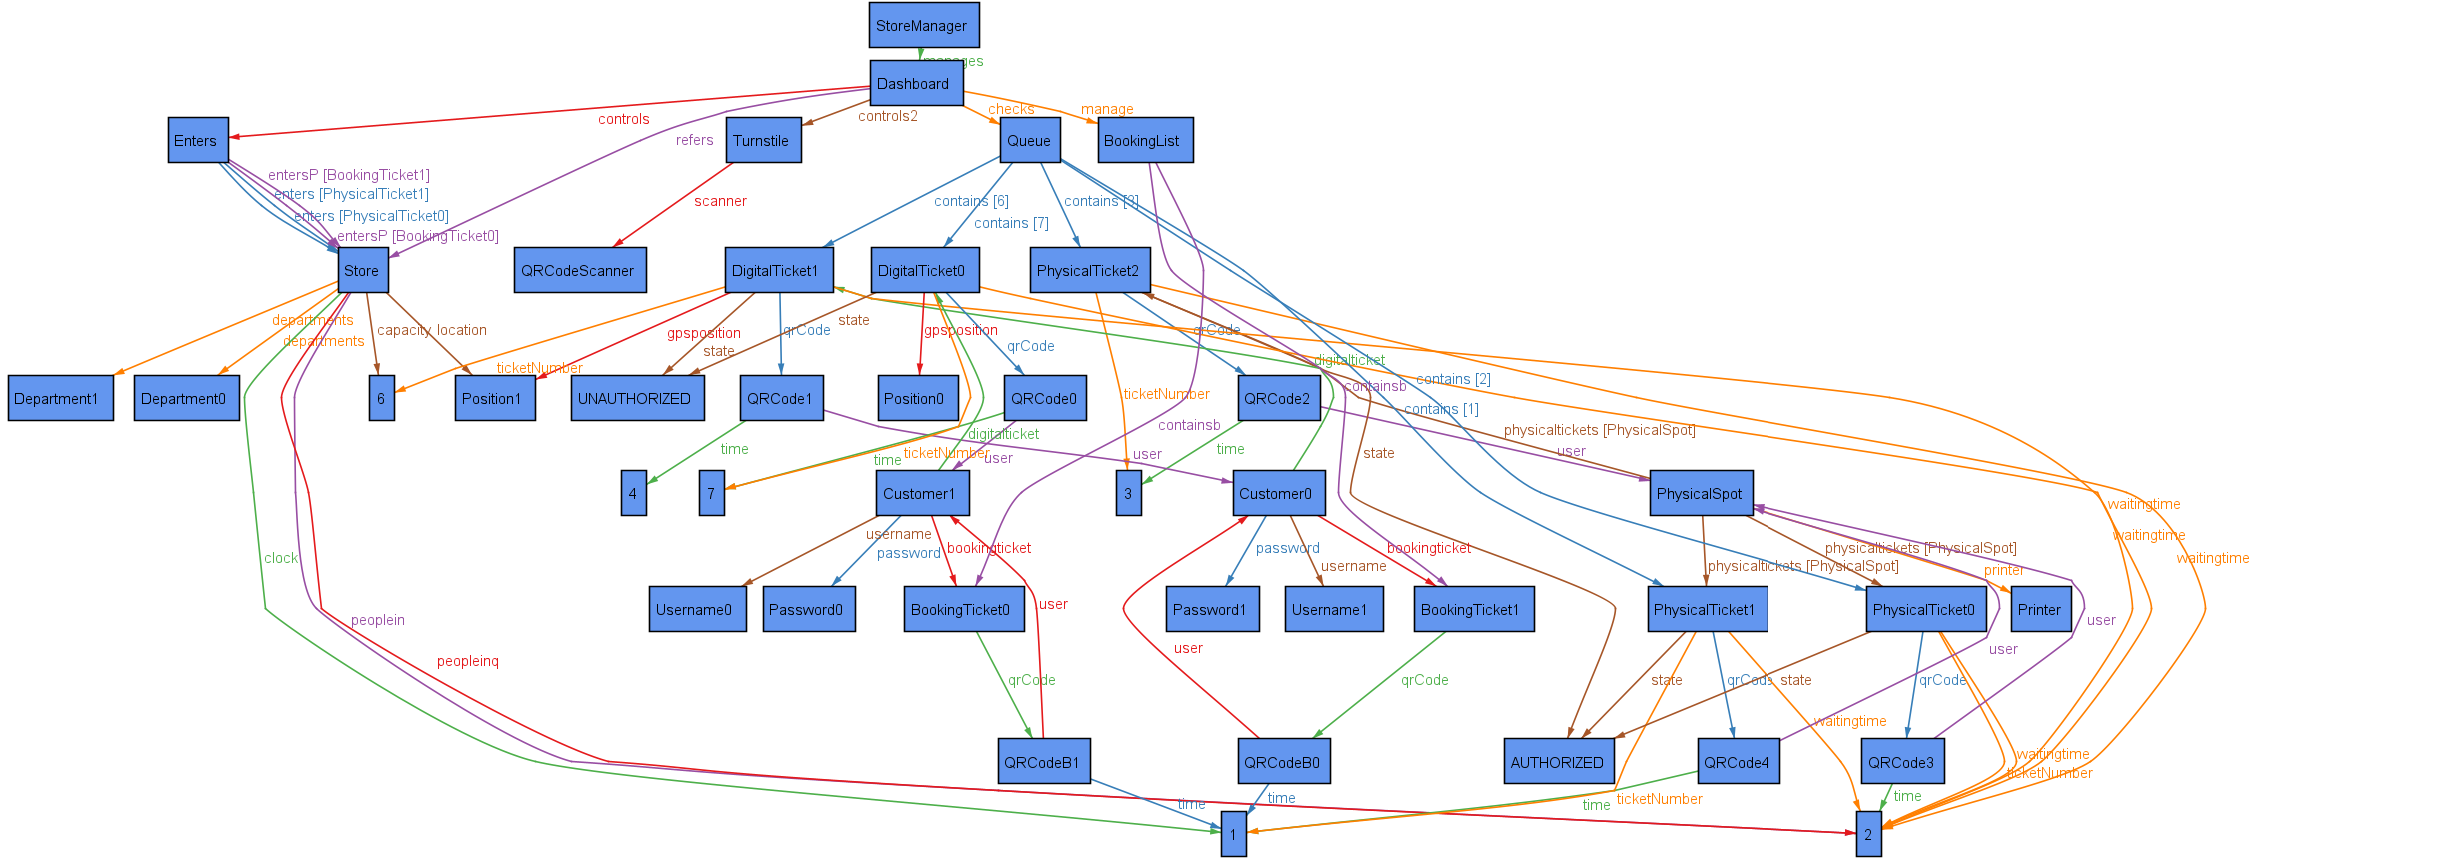
\includegraphics[width=1.0\textwidth]{images/world_3.png}
	\caption{World2.}
	\label{figure: World2}
\end{sidewaysfigure}

\begin{sidewaysfigure}
	\centering
	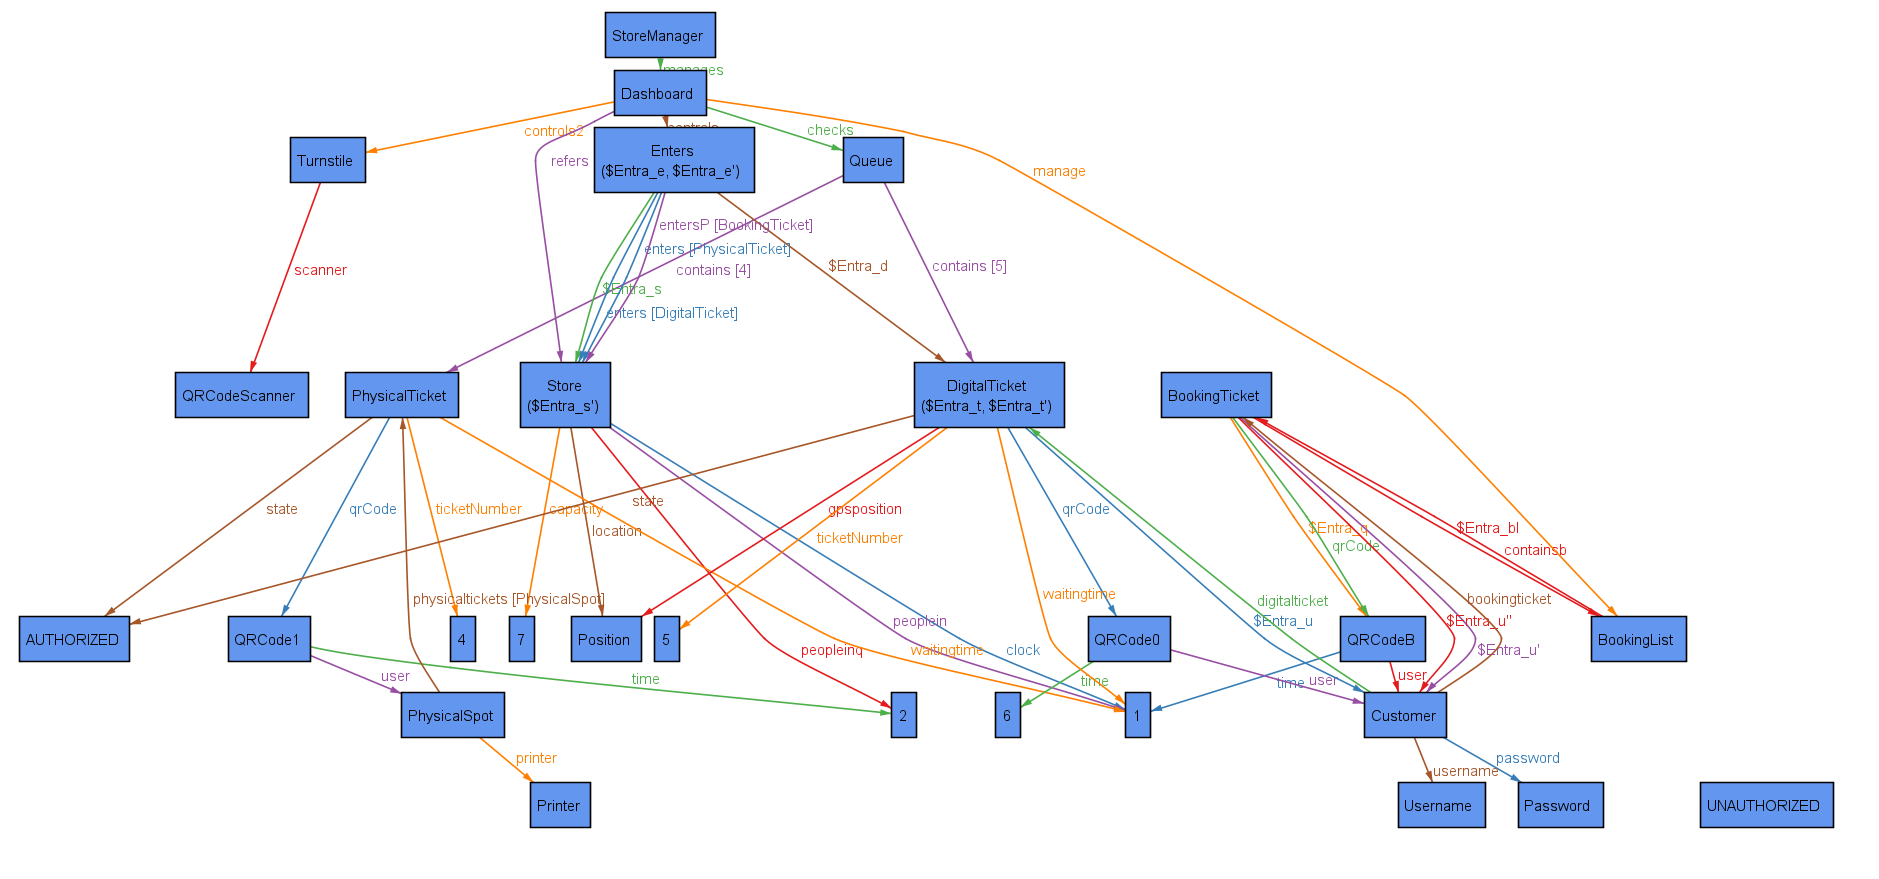
\includegraphics[width=1.0\textwidth]{images/EntraFunction}
	\caption{Entra function.}
	\label{figure: Entra function}
\end{sidewaysfigure}
\chapter{Effort Spent}

\begin{table}[H]
    \centering
    \begin{tabular}{| m{0.8\textwidth} | m{0.2\textwidth} |}
        \hline
        \textbf{Topic}                                                             & \textbf{Hours} \\
        \hline
        Preliminary Discussion                                                     & 6              \\
        \hline
        Introduction                                                               & 4              \\
        \hline
        Product Perspective                                                        & 6              \\
        \hline
        Product Functions                                                          & 1              \\
        \hline
        User Characteristics                                                       & 2              \\
        \hline
        Assumptions, Dependencies and Constraints                                  & 1              \\
        \hline
        External Interface Requirements                                            & 2              \\
        \hline
        Functional Requirements                                                    & 5              \\
        \hline
        Performance Requirements / Design Constraints / Software System Attributes & 5              \\
        \hline
        Alloy Code                                                                 & 12             \\
        \hline
        Revision                                                                   & 4              \\
        \hline
        \hline
        \textbf{Total:}                                                            & 48             \\
        \hline
    \end{tabular}
    \caption{Effort spent by Jas Valencic.}
\end{table}

\begin{table}[H]
    \centering
    \begin{tabular}{| m{0.8\textwidth} | m{0.2\textwidth} |}
        \hline
        \textbf{Topic}                                                             & \textbf{Hours} \\
        \hline
        Preliminary Discussion                                                     & 6              \\
        \hline
        Introduction                                                               & 3              \\
        \hline
        Product Perspective                                                        & 3              \\
        \hline
        Product Functions                                                          & 3              \\
        \hline
        User Characteristics                                                       & 1              \\
        \hline
        Assumptions, Dependencies and Constraints                                  & 2              \\
        \hline
        External Interface Requirements                                            & 8              \\
        \hline
        Functional Requirements                                                    & 10             \\
        \hline
        Performance Requirements / Design Constraints / Software System Attributes & 3              \\
        \hline
        Alloy Code                                                                 & 5              \\
        \hline
        Revision                                                                   & 4              \\
        \hline
        \hline
        \textbf{Total:}                                                            & 48             \\
        \hline
    \end{tabular}
    \caption{Effort spent by Damiano Derin.}
\end{table}
\chapter{References}

\begin{itemize}
    \item Specification document: "R \& DD Assignment AY2020-2021.pdf".
    \item Slides of the lectures.
    \item \glspl{rasd} of past students.
    \item Alloy documentation: "http://alloy.mit.edu/alloy/documentation.html"
    \item Google Maps services: "https://cloud.google.com/maps-platform"
    \item Google Firebase service: "https://firebase.google.com/"
\end{itemize}

%\end{linenumbers}


% bibliogarphy should be moved under References!
%*******************************************************
% Bibliografia
%*******************************************************
\nocite{*}
\bibliography{bib/bibliography}
\bibliographystyle{plain}


\end{document}
